\documentclass[abstract=on,10pt,a4paper,bibliography=totocnumbered]{article}
\usepackage[paper=a4paper,left=35mm,right=35mm,top=25mm,bottom=30mm]{geometry}
\usepackage[doublespacing]{setspace}
\usepackage[english]{babel}
\usepackage[utf8]{inputenc}
\usepackage[round]{natbib}
\usepackage{amsmath}
\usepackage{colortbl}
\usepackage{amsfonts}
\usepackage{amssymb}
\usepackage{gensymb}
\usepackage{graphicx}
\usepackage{tikz}
\usepackage{enumerate}
\usepackage{enumitem}
\usepackage{subcaption}
\usepackage{booktabs}
\usepackage[hidelinks]{hyperref}
\usepackage[nameinlink]{cleveref}
% \usepackage{lineno}
\usepackage{multirow}
\usepackage{arydshln}
\usepackage[flushleft]{threeparttable}
\usepackage[nomarkers, nolists]{endfloat}

%------------------------------------------------------------------------------
%	Some Styling
%------------------------------------------------------------------------------
% Creating some TikZ styles
\tikzset{
  nonterminal/.style = {rectangle
    , minimum size = 6mm
    , very thick
    , draw = black!
  }
}

% Changing the style of captions in figures etc.
\captionsetup{labelfont=bf, format=plain, font=small}

% Change how equations are referenced
\renewcommand{\theequation}{Equation \arabic{equation}}%

%------------------------------------------------------------------------------
%	Titlepage: Header
%------------------------------------------------------------------------------
\title{Step by Step: Using Step Selection Functions to Simulate Dispersal and
Assess Landscape Connectivity}

% \title{Step by Step: The Utility of Dispersal Simulations to Assess Landscape
% Connectivity}

% List of Authors
\author{
  David D. Hofmann\textsuperscript{1,\S} \and
  John W. McNutt\textsuperscript{2} \and
  Arpat Ozgul\textsuperscript{1} \and
  Gabriele Cozzi\textsuperscript{1,2} \and
  Dominik M. Behr\textsuperscript{1,2}
}

% Reduce spacing between authors
\makeatletter
\def\and{%
  \end{tabular}%
  \hskip -0.5em \@plus.17fil\relax
  \begin{tabular}[t]{c}}
\makeatother

% Current Date
\date{\today}

% And here the masterpiece begins
\begin{document}

% Change page numbering
\pagenumbering{gobble}

% Required to be able to cite
\bibliographystyle{apalike}

% Create Titlepage
\maketitle

%------------------------------------------------------------------------------
%	Titlepage: Additional Info
%------------------------------------------------------------------------------
\begin{flushleft}

\vspace{0.5cm}

\textsuperscript{1} Department of Evolutionary Biology and Environmental
Studies, University of Zurich, Winterthurerstarsse 190, 8057 Zurich,
Switzerland.

\textsuperscript{2} Botswana Predator Conservation, Private Bag 13, Maun,
Botswana.

\textsuperscript{\S} Corresponding author (david.hofmann2@uzh.ch)

\vspace{4cm}

\textbf{Running Title:} Release the Dogs! Simulating Wild Dog Dispersal to
Assess Landscape Connectivity

\vspace{0.5cm}

\textbf{Keywords:} dispersal, simulation, movement, integrated step selection,
Kavango-Zambezi Transfrontier Conservation Area, landscape connectivity, Lycaon
pictus

\end{flushleft}

%------------------------------------------------------------------------------
%	Abstract
%------------------------------------------------------------------------------
\newpage
\begin{abstract}
% Dispersal & Connectivity
Dispersal is an important process that allows species to avoid inbreeding,
colonize new habitats and reinforce non-viable subpopulations. Successful
dispersal thus represents a crucial pre-requisite for long-term species
persistence in wild animal populations. However, the ability to disperse is
contingent a sufficient degree of landscape connectivity, which is why the
estimation of connectivity and preservation of dispersal corridors has become a
task of extraordinary importance for conservation authorities.

% Quantifying Connectivity
Over the past two decades, ecologists have primarily relied on analytical tools
such as least-cost analysis and circuit theory to model and investigate
landscape connectivity. Despite their usefulness for a diverse suite of
ecological applications, both methods make several restricting assumptions that
limit their usefulness in reality. Individual-based dispersal simulations have
been proposed to address these shortcomings, yet due to the sheer amount of
non-trivial modeling decisions decisions, a unified and objective framework to
simulate dispersal is missing.

% Step Selection Functions
Recent innovations in movement ecology have brought forward novel opportunities
to study animal dispersal and estimate landscape connectivity. In particular,
the rich suite of resource selection functions, namely point-, step-, and
path-selection functions, have undergone substantial improvements over the past
years. Most notably, step-selection functions have been generalized to
\textit{integrated} step selection functions, which essentially represent fully
mechanistic movement models based on which an individual's movement could be
simulated. While such models have been applied to study \textit{steady-state}
utilization distribution resident animals, a similar approach may be useful to
investigate \textit{transient} movement behavior during dispersal and landscape
connectivity.

% Current Study
Here, we showcase the use of integrated step selection functions as simple,
individual-based, and spatially explicit movement model to simulate dispersal of
the endangered African wild dog across the world's largest transboundary
conservation area, the Kavango-Zambezi Transfrontier Conservation Area
(KAZA-TFCA). For this, we utilize data collected on 16 dispersing wild dog
coalitions in combination with relevant habitat covariates. We analyse the data
using integrated step selection functions, thereby parametrizing a fully
mechanistic movement model describing how dispersing wild dogs move through the
available landscape. Based on this model, we simulate 80'000 dispersers moving
across the extent of the KAZA-TFCA and generate a set of three connectivity
maps, each focused on a different aspect of connectivity. Finally, we discuss
the benefits and pitfalls of such a simulation-based approach and highlight
potential improvements to be made in the future.

\end{abstract}

%------------------------------------------------------------------------------
%	Main Text
%------------------------------------------------------------------------------
\newpage

\onehalfspacing
\tableofcontents
\doublespacing

% Change page numbering
\newpage
\pagenumbering{arabic}

% Create linenumbers
% \linenumbers

\section{Introduction}

% Importance of Dispersal & Connectivity
\subsection{Importance of Dispersal \& Connectivity (90\%)}
Dispersal is defined as the movement of individuals away from their natal
location to the site of first reproduction \cite{Howard.1960}. It is a vital
process governing the social structure of wild animal populations that are
distributed in space \citep{Hanski.1998, Clobert.2012} and may strongly affect
population dynamics at different spatial and social scales \citep{Hanski.1999a,
Clobert.2012}. Dispersal allows species to maintain genetic diversity
\citep{Perrin.1999, Perrin.2000, Frankham.2002, Leigh.2012, Baguette.2013}, to
rescue small, non-viable populations \citep{Brown.1977}, and to promote the
colonization or recolonization of unoccupied habitats \citep{Hanski.1999b,
MacArthur.2001}. However, successful dispersal requires a sufficient degree of
landscape connectivity \citep{Fahrig.2003, Clobert.2012}, which is why the
identification and protection of major dispersal corridors has become a
fundamental task in conservation science \citep{Nathan.2008, Doerr.2011,
Rudnick.2012}. The ability to pinpoint relevant dispersal hotspots requires
information on movement behavior during dispersal and knowledge about factors
that limit dispersal and therefore connectivity \citep{Baguette.2013,
Vasudev.2015}.

% Advancements in GPS Technology & Movement Ecology
\subsection{Advancements in GPS Technology \& Movement Ecology (90\%)}
Thanks to novel technologies developed over the past decades, particularly of
GPS/Satellite radio-collars, the use of GPS data to study animal dispersal and
connectivity has accelerated \citep{Elliot.2014, Jonsson.2016, Williams.2019}.
Additionally, the advent of publicly accessible satellite imagery and
sophisticated remote sensing techniques to represent the physical landscape
through which individuals disperse have heralded a ``golden age of animal
tracking'' \citep{Kays.2015}. Concurrently, the availability of large amounts of
empirical data and an increased computational power have led to the development
of numerous techniques to study dispersal and highlight critical corridors
between subpopulations \citep{Boyce.2002, Fortin.2005, Cushman.2010,
Zeller.2012, Diniz.2020}.

% Resource Selection & Connectivity
\subsection{Resource Selection \& Connectivity (90\%)}
\textit{Resource selection functions} \citep{Boyce.2002} and derived methods
such as \textit{step selection functions} \citep{Fortin.2005} and \textit{path
selection functions} \citep{Cushman.2010} have proven particularly useful for
studying animal movement \citep{Fieberg.2020} and modeling connectivity
\citep{Diniz.2020}. These methods allow estimating habitat preferences of the
focal species by comparing covariates at locations visited by the animal to the
same covariates at locations available to, but not visited by the animal
\citep{Boyce.2002, Fortin.2005, Cushman.2010, Thurfjell.2014}. The so estimated
preferences can then be used to predict a permeability surface, indicating the
expected ease at which an animal can traverse a given area \citep{Spear.2010,
Zeller.2012, Etherington.2016}. Ultimately, the permeability surface serves as
input to a connectivity model that is used to reveal movement corridors
\citep{Diniz.2020}. Two of the most prominent connectivity models are least-cost
analysis (LCPA; \citealp{Adriaensen.2003}) and circuit theory (CT;
\citealp{McRae.2006, McRae.2008}), both graph-based methods that estimate
conductance of the landscape to infer likely movement corridors. Despite their
intuitive nature and ease of use, both methods make rigorous assumptions about
animal movement that are often not fulfilled in reality \citep{Diniz.2020}.

% Issues with Least-Cost Paths
\subsection{Issues with Least-Cost Paths (90\%)}
In LCP analysis, for instance, a least costly path always exists, even if
associated movement costs are unreasonably high and will never be incurred by a
dispersing individual. The method also presumes that animals have an infinite
perceptual range and a preconceived end-point in mind, such that they choose a
cost-minimizing route accordingly. These assumptions may be fulfilled by
migrating animals that typically move between a discrete set of habitats through
familiar landscapes. Dispersers, on the other hand, usually move over long
distances into unknown territory and are therefore less likely to be aware of
associated movement costs \citep{Koen.2014, Abrahms.2017, Cozzi.2020}. Another
issue of LCPs analysis concerns the fact that least-costly routes, by their very
nature, are only one pixel wide \citep{Pinto.2009}. This neglects the fact that
alternative routes with similar costs may exist and implies that the width of
inferred movement routes depends on the resolution of chosen covariate layers
and may not be biologically meaningful \citep{Diniz.2020}. Although some of
these deficiencies can be addressed using less stringent versions of the least
cost algorithm (e.g. least-cost \textit{corridors} \citep{Pinto.2009},
\textit{thresholded} least-cost paths \citep{Landguth.2012}, and
\textit{randomized} least-cost paths \citep{Panzacchi.2016, VanMoorter.2021}), a
certain degree of arbitrariness remains.

% Issues with Circuit Theory
\subsection{Issues with Circuit Theory (90\%)}
CT entails similarly unreasonable restrictions that are rarely ever met. For
example, because CT only allows movements from a source cell to its four or
eight adjacent cells, it implicitly posits that animals exhibit a perceptual
range of a single pixel. Given that covariate layers are usually resolved with a
pixel size between 30 m x 30 m and 1 km x 1 km, this hardly ever renders the
true capability of animals to perceive the environment. Moreover, CT is built
around the assumption of a complete random walk \citep{Diniz.2020}, entailing
that directional biases cannot be rendered. Nevertheless, directionality is a
common characteristic in animal movement \citep{Bovet.1991, Schultz.2001},
especially in dispersing individuals \citep{Cozzi.2020, Hofmann.2021}.

% Issues with Both Methods
\subsection{Issues of Both Methods}
Finally, neither LCP analysis nor CT are capable of rendering the temporal
dimension of dispersal \citep{Diniz.2020}. Statements about the expected
duration required to traverse a certain corridor are therefore impossible.
Likewise, because movement is not modeled explicitly, interactions between
movement and habitat preferences of the focal species cannot be rendered.
Connectivity therefore merely arises in result to the landscape structure, which
is usually referred to as structural connectivity. While structural connectivity
yields insights in the \textit{potential} of the landscape to be traversed, it
does not enable to quantify the \textit{actual} gene flow through the area.
Consequently, a functional view on connectivity, which also renders the
behavioral response of the animal with respect to prevailing habitat conditions,
is often more desirable \citep{Tischendorf.2000, Baguette.2013}.

% What about IBMMs?
\subsection{What about IBMMs? (90\%)}
To address the issues inherent to LCPs and CT, individual-based movement models
(IBMMs) have been proposed and applied \citep{Diniz.2020}. In these models,
dispersal trajectories are simulated spatially explicitly, based on movement
rules that determine how individuals move over and interact with the prevailing
landscape \citep{Gustafson.1996, Gardner.2004, Graf.2007, KramerSchadt.2004,
Revilla.2004, Revilla.2008, Kanagaraj.2013, Clark.2015, Allen.2016,
Hauenstein.2019, Zeller.2020, Vasudev.2021}. Using the simulated trajectories,
one can calculate a set of connectivity metrics, such as inter-patch
connectivity and traversal frequency, to reveal major dispersal corridors
\citep{Kanagaraj.2013, BastilleRousseau.2018, Hauenstein.2019, Zeller.2020}.
However, while IBMMS can be employed to overcome any of the shortcomings
intrinsic to LCPs and CT, they are subject to a vast amount of subjective,
non-trivial modeling decisions. Moreover, they can be challenging to fit and
require vast amounts of movement data, ideally collected during dispersal
\citep{Diniz.2020}. Consequently, alternative methods that require fewer
modeling decisions and are straight forward to apply are desirable.

% Step Selection Analysis
\subsection{Step Selection Analysis (90\%)}
Here, we investigate the usefulness of integrated step selection functions
(ISSFs, \citealp{Avgar.2016}), as a relatively simple but powerful IBMM based on
which dispersal can be simulated. While regular SSFs were intended to learn
about relative habitat preferences of the focal species \citep{Fortin.2005,
Thurfjell.2014, Avgar.2017}, the method has recently been generalized to
\textit{integrated} SSFs and now enables to jointly study habitat and movement
preferences, as well as potential interactions between them \citep{Avgar.2016,
Signer.2017, Fieberg.2020}. ISSFs therefore provide a relatively simple means to
model complex movement behavior, where movement is viewed as the result of two
intertwined behavioral kernels (e.g. \citealp{Prokopenko.2017, Munden.2020}).
Importantly, a parametrized ISSF model can be employed as a fully mechanistic
movement model based on which individual movement trajectories can be simulated
\citep{Avgar.2016, Signer.2017}. In fact, \cite{Signer.2017} used ISSF to
simulate steady state utilization distributions of resident animals that were
moving around a point of attraction. However, the degree to which such
simulations are helpful in detecting movement corridors and modeling landscape
connectivity remains to be investigated.

% Study Species & Study Area
\subsection{Study Species \& Study Area (90\%)}
One of the species for which long-term viability relies on sufficient landscape
connectivity is the endangered African wild dog \textit{Lycon pictus}. While
once present across entire sub-Saharan Africa, wild dogs have disappeared from a
vast majority of their historic range due to persecution by humans, habitat
fragmentation and destruction, and deadly diseases \citep{Woodroffe.2012}. As of
today, only 6'000 free-ranging individuals remain in small and spatially
scattered subpopulations \citep{Woodroffe.2012}. Within those subpopulations,
wild dogs form cohesive packs comprising 8 to 12 adults and their offspring
\cite{McNutt.1995}. After reaching sexual maturity, male and female offspring
form same-sex coalitions and disperse from their natal pack in search for
potential mating partners and a suitable territory to settle \citep{McNutt.1996,
Behr.2020}. New packs are formed when dispersing coalitions join unrelated
opposite-sex dispersing coalitions \citep{McNutt.1996}. Dispersing wild dogs can
cover several hundred kilometers across a variety of landscapes
\citep{DaviesMostert.2012, Masenga.2016, Cozzi.2020, Hofmann.2021}. One of the
few strongholds for this species lies near the Moremi Game Reserve in northern
Botswana, which is part of the world's largest transboundary protected area,
namely the Kavango-Zambezi Transfrontier Conservation Area (KAZA-TFCA). This
area has originally been intended to facilitate migration of elephants, but is
expected to provide benefits to a multitude of other species \citep{Elliot.2014,
Brennan.2020, Hofmann.2021}.

% Previous Paper
\subsection{Previous Paper (90\%)}
In a previous study, we assessed landscape connectivity for dispersing African
wild dogs within the KAZA-TFCA using least-cost methods \citep{Hofmann.2021}.
Specifically, we fitted a basic habitat selection model and predicted a
permeability surface that we used to compute least-cost paths and corridors. We
now expand on this knowledge and use ISSFs to develop a more mechanistic
movement model of dispersing wild dogs (\Cref{GraphicalAbstract}). We employ the
model to simulate dispersers moving across the KAZA-TFCA and generate three
distinct connectivity maps, each shedding light onto a different aspect of
connectivity. With this work, we exemplify how ISSFs can be utilized for
dispersal simulations and we discuss several benefits of this approach over
traditional connectivity modeling techniques such as least-cost analysis and
circuit theory. Most importantly, simulations based on ISSFs provide a more
generic view on how connectivity emerges and to which degree connectivity
depends on the dispersal duration. In addition, by generating proper dispersal
trajectories, network theory can be applied to calculate network metrics that
are pertinent to connectivity analysis.

\begin{figure}[htbp]
  \begin{center}
    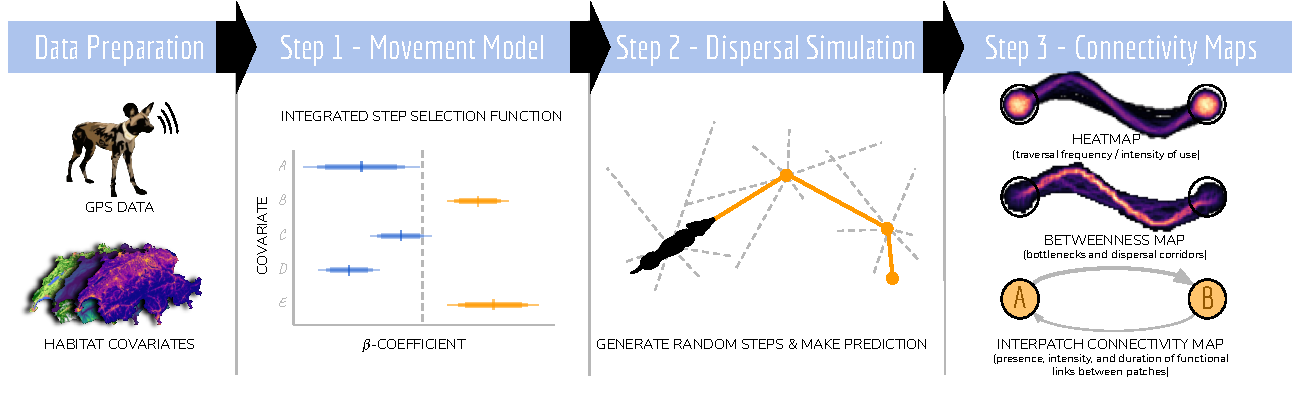
\includegraphics[width = \textwidth]{99_GraphicalAbstract.pdf}
    \caption{Flowchart of the simulation-based connectivity analysis as proposed
    in this article. First, GPS data and habitat covariates have to be
    collected. The combined data is then analyzed in an integrated step
    selection model, which enables the parametrization of the focal species'
    habitat and movement kernels. The parametrized model is then treated as an
    individual-based movement model and used to simulate dispersal trajectories.
    Ultimately, simulated trajectories serve to produce a set of maps that are
    pertinent to landscape connectivity. This includes a heatmap, indicating the
    relative traversal frequency across the study area, a betweenness map,
    highlighting movement corridors and bottlenecks, and, finally, an
    inter-patch connectivity map, where the frequency of connections and their
    average duration can be depicted. \textcolor{red}{Photos: Whom to cite?
    Vectronics or Photographers?}}
    \label{GraphicalAbstract}
  \end{center}
\end{figure}

\section{Methods}
\subsection{Study Area (90\%)}
The study area was defined by a bounding box centered at -17\degree 13'9''S,
23\degree 56'4''E (\Cref{StudyArea}a) stretching over 1.3 Mio.
km\textsuperscript{2} and encompassed the entire KAZA-TFCA (\Cref{StudyArea}b).
The KAZA-TFCA represents the world's largest transboundary conservation area and
comprises parts of Angola, Botswana, Namibia, Zimbabwe, and Zambia. It covers a
total of 520'000 km\textsuperscript{2} and hosts diverse landscapes, ranging
from savanna to grassland and from dry to moist woodland habitats. In its center
lies the Okavango Delta, a dominant hydrogeographical feature and the world's
largest flood-pulsing inland delta. The wet season within the KAZA-TFCA lasts
from November to March and is out of phase with the flood in the Okavango Delta,
which peaks between July and August \citep{McNutt.1996, Wolski.2017}. Although
large portions within the KAZA-TFCA are designated national parks or other
protected areas, considerable human influence remains due to roads, agricultural
sites and settlements and villages that are distributed across the KAZA-TFCA's
landscape.

\begin{figure}[h]
  \begin{center}
    \begin{tikzpicture}
        \node[anchor=south west,inner sep=0] (image) at (0,0,0) {
        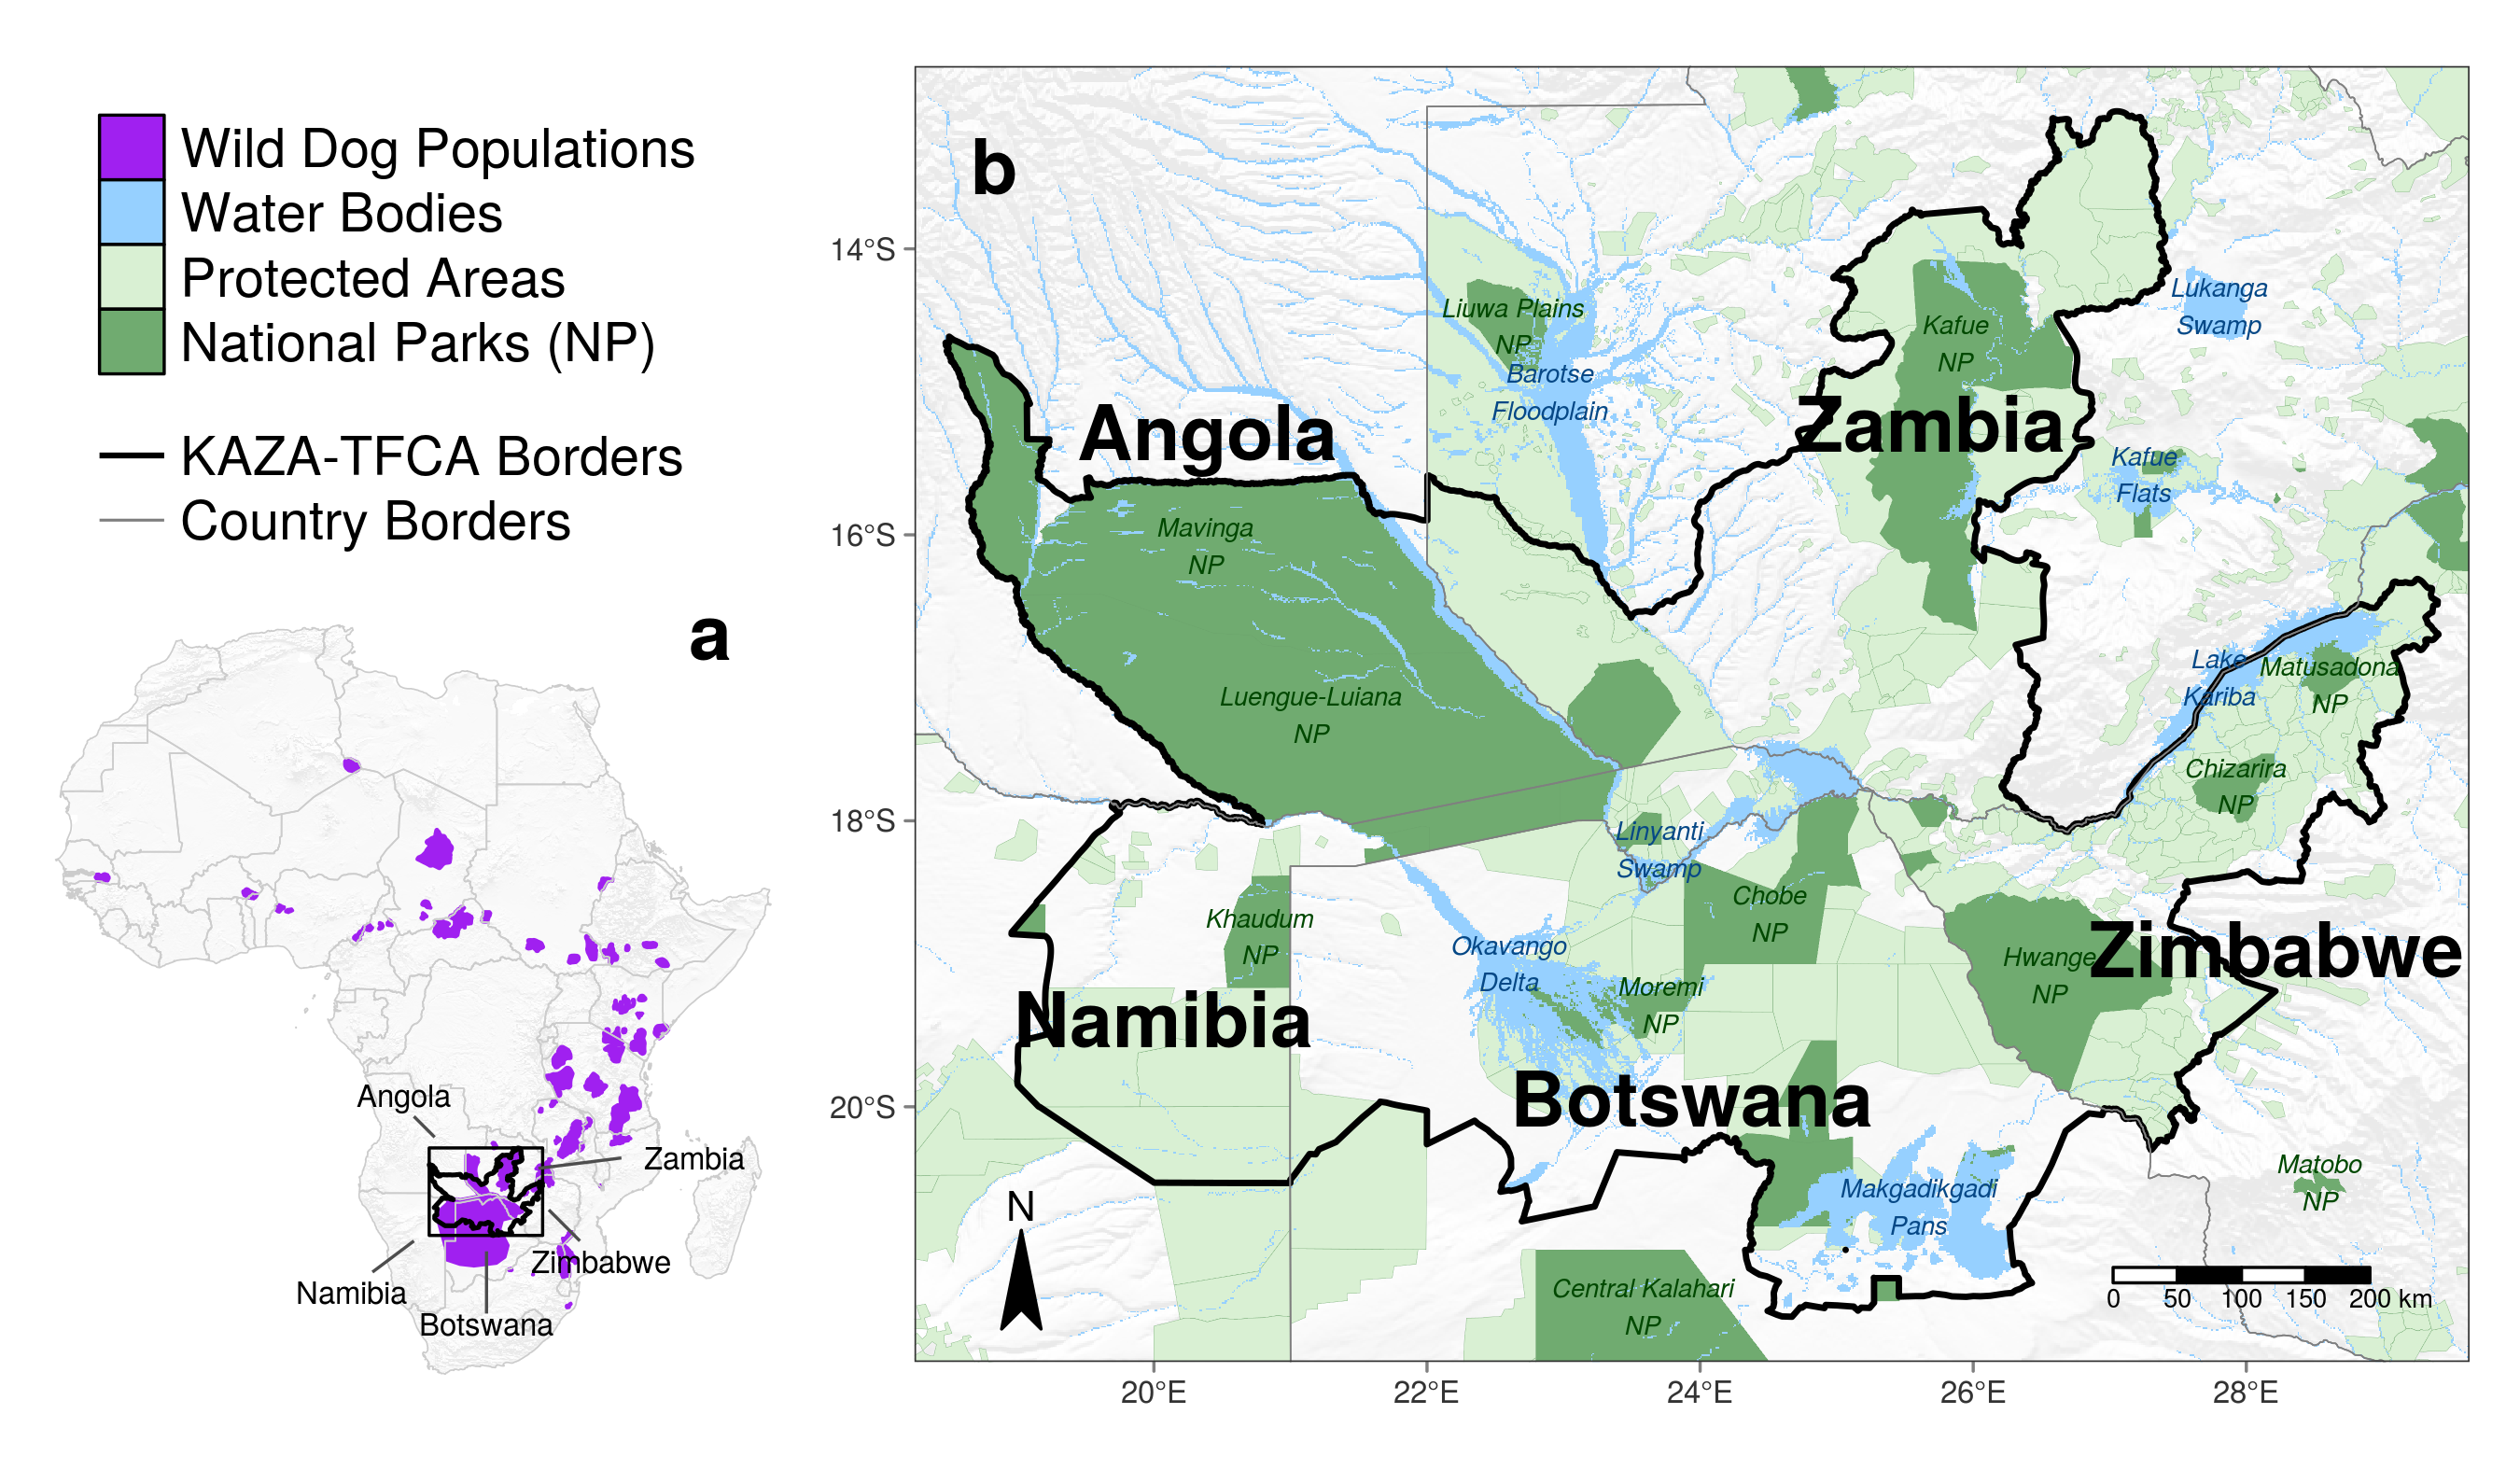
\includegraphics[width=\textwidth]{99_StudyArea.png}
        };
        \begin{scope}[x={(image.south east)},y={(image.north west)}]
            % % next four lines will help you to locate the point needed by forming a grid.
            % % comment these four lines in the final picture.
            % \draw[help lines,xstep=.1,ystep=.1] (0,0) grid (1,1);
            % \draw[help lines,xstep=.05,ystep=.05] (0,0) grid (1,1);
            % \foreach \x in {0,1,...,9} { \node [anchor=north] at (\x/10,0) {0.\x}; }
            % \foreach \y in {0,1,...,9} { \node [anchor=east] at (0,\y/10) {0.\y};}
            % % upto here
            \draw[densely dotted, black] (0.169, 0.222) -- (0.364, 0.955);
            \draw[densely dotted, black] (0.169, 0.157) -- (0.364, 0.074);
        \end{scope}
    \end{tikzpicture}
    \caption{Illustration of the study area located in southern Africa. (a) The
    study area was confined by a bounding box spanning the entire KAZA-TFCA and
    encompassed parts of Angola, Namibia, Botswana, Zimbabwe, and Zambia. (b)
    The KAZA-TFCA represents the world's largest terrestrial conservation area
    and covers a total of 520'000 km\textsuperscript{2}. Its purpose is to
    re-establish connectivity between already-existing national parks (dark
    green) and other protected areas (light green).}
    \label{StudyArea}
  \end{center}
\end{figure}

\subsection{GPS Relocation Data (90\%)}
Between 2011 and 2019, we collected GPS relocation data on dispersing wild dogs
from a free-ranging wild dog population inhabiting the Moremi National Park in
northern Botswana \citep{Cozzi.2020, Hofmann.2021}. We selected potential
dispersers based on age, pack size, number of same‐sex siblings within the pack,
and presence of unrelated opposite-sex individuals in the pack
\citep{McNutt.1996, Behr.2020}. We immobilized selected individuals using a
cocktail of Ketamine/Xylazine/Atropine \citep{Osofsky.1996, Cozzi.2020} that was
injected by dart, fired from a CO\textsubscript{2}-pressurized gun
(\textit{DAN-Inject, Denmark}). Immobilized individuals were fitted with
GPS/Satellite radio collars (\textit{Vertex Lite; Vectronic Aerospace GmbH,
Berlin}) that guaranteed automated drop-off through a decomposable piece of
cotton. Handling and collaring of all individuals was supervised by a
Botswana-registered wildlife veterinarian and all individuals quickly rejoined
their pack after immobilization.

16 collared individuals eventually dispersed, each in a separate same-sex
dispersal coalition (7 female and 9 male coalitions). During dispersal, collars
were programmed to record a GPS fix every 4 hours, all of which were regularly
transmitted over the Iridium satellite system, thereby allowing to remotely
track individuals, even if they left the main study area and crossed
international borders. Because behavior during dispersal is more pertinent for
assessing landscape connectivity \citep{Elliot.2014, Abrahms.2017}, we discarded
all data that was collected during residency and only retained GPS data recorded
during dispersal. In some instances, exact dispersal dates were known from field
observations, whereas in other cases we determined dispersal phases using the
net-squared displacement metric. Net squared displacement measures the squared
Euclidean distance of a GPS relocation to a reference point \citep{Borger.2012},
which in our case was set to the center of each individual's natal home range.
Thus, dispersal was deemed to have started when an individual left its natal
home range and ended once individuals became sedentary again. As previous
research found no differences in behaviors of females and males during dispersal
\citep{Woodroffe.2019, Cozzi.2020}, we did not distinguish between sexes. After
collection, we converted collected GPS coordinates (n = 4'169) to steps, where
each step represented the straight-line distance traveled by an individual
between two consecutive GPS relocations \citep{Turchin.1998}. To ensure a
regular sampling interval, we removed fixes that were not successfully collected
on the 4-hourly schedule (\( \pm \) 15 minutes).

\subsection{Covariates (90\%)}
We represented the physical landscape across the study area using a set of
habitat covariates that included water-cover, distance to water, woodland-cover,
and shrub/grassland-cover. Because water cover greatly changes within and
between years in the Okavango Delta, we applied a remote sensing algorithm and
generated frequently updated water cover layers and corresponding distance to
water layers (see \citealp{Wolski.2017} and Appendix A3 in
\citealp{Hofmann.2021}). Resulting water layers thus temporally aligned with our
dispersal events. We furthermore computed a proxy for human influence, rendering
anthropogenic pressures stemming from human-density, agricultural sites, and
roads. All spatial layers were coarsened or interpolated to a target resolution
of 250 m by 250 m. Further details on the sources and preparation of each
habitat covariate are given in \cite{Hofmann.2021}.

Besides habitat covariates, we computed movement metrics that we used as
movement covariates in our models. Movement metrics were calculated for each
step and included the step length (\textsf{sl}), its natural logarithm
(\textsf{log(sl)}), and the cosine of the relative turning angle
(\textsf{cos(ta)}) (for details see \citep{Avgar.2016, Fieberg.2020}). Because
wild dogs follow a diurnal activity pattern \citep{Castello.2018}, we also coded
a binary variable (\textsf{LowActivity}) indicating whether a step was realized
during periods of low wild dog activity (17:00 to 09:00 local time) or high wild
dog activity (09:00 to 17:00 local time). Handling and manipulation of all data,
as well as all models and simulations were implemented with the statistical
software {\tt R}, version 3.6.6 \citep{R.2019}. Several helper functions were
written in {\tt C++} and imported into {\tt R} using the {\tt Rcpp} package
\citep{Eddelbuettel.2011, Eddelbuettel.2013}

\subsection{Movement Model (80\%)}
We used ISSFs to parametrize a mechanistic movement model for dispersing wild
dogs \citep{Avgar.2016}. To conduct ISSF analysis, we paired each realized step
with 24 random steps. An observed step plus its 24 random steps formed a stratum
and received a unique identifier. As suggested by \cite{Avgar.2016}, we
generated random steps by sampling random turning angles from a uniform
distribution (\(-\pi, +\pi\)) and step lengths from a gamma distribution that
was fitted to realized steps (scale = 6'308, shape = 0.37). Along each step, we
extracted and averaged spatial covariates using the {\tt velox} package
\citep{Hunziker.2021}. We also calculated the movement metrics \textsf{sl},
\textsf{log(sl)}, and \textsf{cos(ta)} for each observed and random step. To
facilitate model convergence, we standardized all continuous covariates to a
mean of zero and a standard deviation of one. Since correlation among covariates
was low (\(|r| > 0.6\); \citealp{Latham.2011}), we retained all of them for
modeling.

To contrast realized steps (scored 1) and random steps (scored 0), we assumed
that animals assigned a selection score \(w(x)\) of the exponential form to each
step \citep{Fortin.2005}. The selection score \(w(x)\) of each step thus
depended on its associated covariates (\(x_1, x_2, ..., x_n\)) and on the
animal's preferences (i.e. relative selection strengths; \citealp{Avgar.2017})
towards these covariates (\(\beta_1, \beta_2, ..., \beta_n\)):

\begin{equation}
\label{EQ1}
  w(x) = exp(\beta_1 x_1 + \beta_2 x_2 + ... + \beta_n x_n)
\end{equation}

The probability of a step being realized was then contingent on the step's
selection score, as well as on the selection scores of all other step in the
same stratum:

\begin{equation}
\label{EQ2}
  P(Y_{i} = 1 | Y_{1} + Y_{2} + ... + Y_{i} = 1) =
  \frac{w(x_{i})}{w(x_{1}) + w(x_{2}) + ... + w(x_{i})}
\end{equation}

We ran conditional logistic regression analysis in the r-package {\tt glmmTMB}
to estimate preferences of interest. To handle multiple individuals, we applied
the mixed effects technique developed by \citep{Muff.2020}, which allows to
effectively model random slopes. Thus, we treated animal IDs as random effect
and modeled random slopes for each covariate.

The structure of the movement model was based on the habitat selection model for
dispersing wild dogs presented in \cite{Hofmann.2021}. In the original model
(referred to as base model hereafter), no interactions between habitat
covariates (\textsf{Water, DistanceToWater\textsuperscript{0.5}, Woodland,
Shrubs/Grassland, Human Influence}) and movement covariates (\textsf{sl,
log(sl), cos(ta)}) were considered. Hence, we slightly expanded this base model
and proposed interactions between all movement and habitat covariates. More
specifically, we started with the base model and incrementally increased model
complexity by adding all possible two-way interactions between habitat
covariates and movement covariates. For instance, for the covariate
\textsf{Water}, we proposed the interactions \textsf{Water:log(sl)},
\textsf{Water:log(sl)}, and \textsf{Water:cos(ta)}. Besides those combinations,
we also proposed the interactions \textsf{sl:cos(ta)} and
\textsf{log(sl):cos(ta)} to account for a correlation between turning angles and
step lengths, as well as the interactions \textsf{sl:LowActivity} and
\textsf{log(sl):LowActivity} to account for the fact that step lengths may
differ due to wild dogs' diurnal activity pattern. To compare competing models
and assess the most parsimonious movement model, we ran stepwise forward model
selection based on Akaike's Information Criterion (AIC, \citealp{Burnham.2002}).

We validated the predictive power of the most parsimonious movement model using
k-fold cross-validation for case-control studies as suggested by
\cite{Fortin.2009}. For this, we randomly assigned 80\% of the strata to a
training set and the remaining 20\% to a testing set. Using the training data we
parametrized a movement model based on which we predicted selection scores
\(w(x)\) for all steps in the test data. Within each stratum, we then assigned
ranks 1-25 to each step based on predicted selection scores, where rank 1 was
given to the step with the highest score \(w(x)\). Across all strata we
determined the realized step's rank and we calculated rank frequencies of
realized steps across all strata. Finally, we computed Spearman's rank
correlation between ranks and associated frequencies \(r_{s, realized}\). We
replicated the entire procedure 100 times and computed the mean correlation
coefficient (\(\bar{r}_{s, realized}\)), as well as its 95\% confidence interval
across all replicates. For comparison, we repeated the same procedure 100 times
assuming random preferences, which we implemented by discarding the realized
step from all strata and identifying the rank of a random step in each stratum.
Again, we calculated Spearman's rank correlation coefficient (\(r_{s,
random}\)), its mean across repetitions (\(\bar{r}_{s, random}\)), and its 95\%
confidence interval. This validation ultimately proofs a significant prediction
in case the confidence intervals of \(\bar{r}_{s, realized}\) and \(\bar{r}_{s,
random}\) do not overlap.

\subsection{Dispersal Simulation (80\%)}
We used the most parsimonious movement model to simulate 80'000 virtual
dispersers moving across the KAZA-TFCA. The simulation resembled an inverted
ISSF and was set up as follows. (1) We defined a random source point and assumed
a random initial orientation of the animal. (2) Departing from the source point,
we generated 25 random steps by sampling turning angles from a uniform
distribution (\(-\pi, +\pi\)) and step lengths from our fitted gamma
distribution. Similar to the input data, each random step represented the
straight line movement within 4 hours. To prevent unreasonably large steps, we
capped sampled step lengths to a maximum of 35 km, which corresponded to the
farthest distance ever traveled within 4 hours by one of our dispersers. (3)
Along each random step, we extracted and averaged habitat covariates and we
calculated movement covariates. To ensure compatible scales, we standardized
extracted values using the same parameters applied to our input data. (4) We
applied the parametrized movement model to predict the selection score \(w(x)\)
for each step and we translated predicted scores into probabilities using
\Cref{EQ2}. (5) We sampled one of the random steps based on predicted
probabilities and determined the animal's new position. We repeated steps (2) to
(5) until 2'000 steps were realized, implying a total 160 Mio. simulated steps.

To minimize the influence of edge effects and to deal with random steps leaving
the study area, we followed \citep{Koen.2010} and artificially expanded all
covariate layers by adding a 100 km wide buffer zone. Within the buffer zone, we
randomized covariate values by resampling values from the original covariate
layers. Through this buffer zone, simulated dispersers were able to leave and
re-enter the main study area. In cases where proposed random steps transgressed
the border of this buffer zone, we resampled transgressing steps until they
fully lied within the buffer, thereby forcing simulated individuals to ``bounce
off'' such invisible borders.

\subsection{Source Points (90\%)}
We released 80'000 virtual dispersers from 80'000 unique source points
distributed across the study area. 50'000 virtual dispersers were released from
randomly selected source points within contiguous protected areas larger \(>\)
700 km\textsuperscript{2} (\Cref{SourcePoints}a), which conforms to average home
range requirements of resident wild dogs \citep{Pomilia.2015} and allowed us to
remove patches too small to host viable populations. By distributing source
points randomly, the number of source points per km\textsuperscript{2} was
approximately equal within protected areas. To render potential immigrants into
the study system, we released another 30'000 dispersers at random locations
inside the 100 km wide buffer zone surrounding the main study area
(\Cref{SourcePoints}b).

\begin{figure}[htbp]
  \begin{center}
    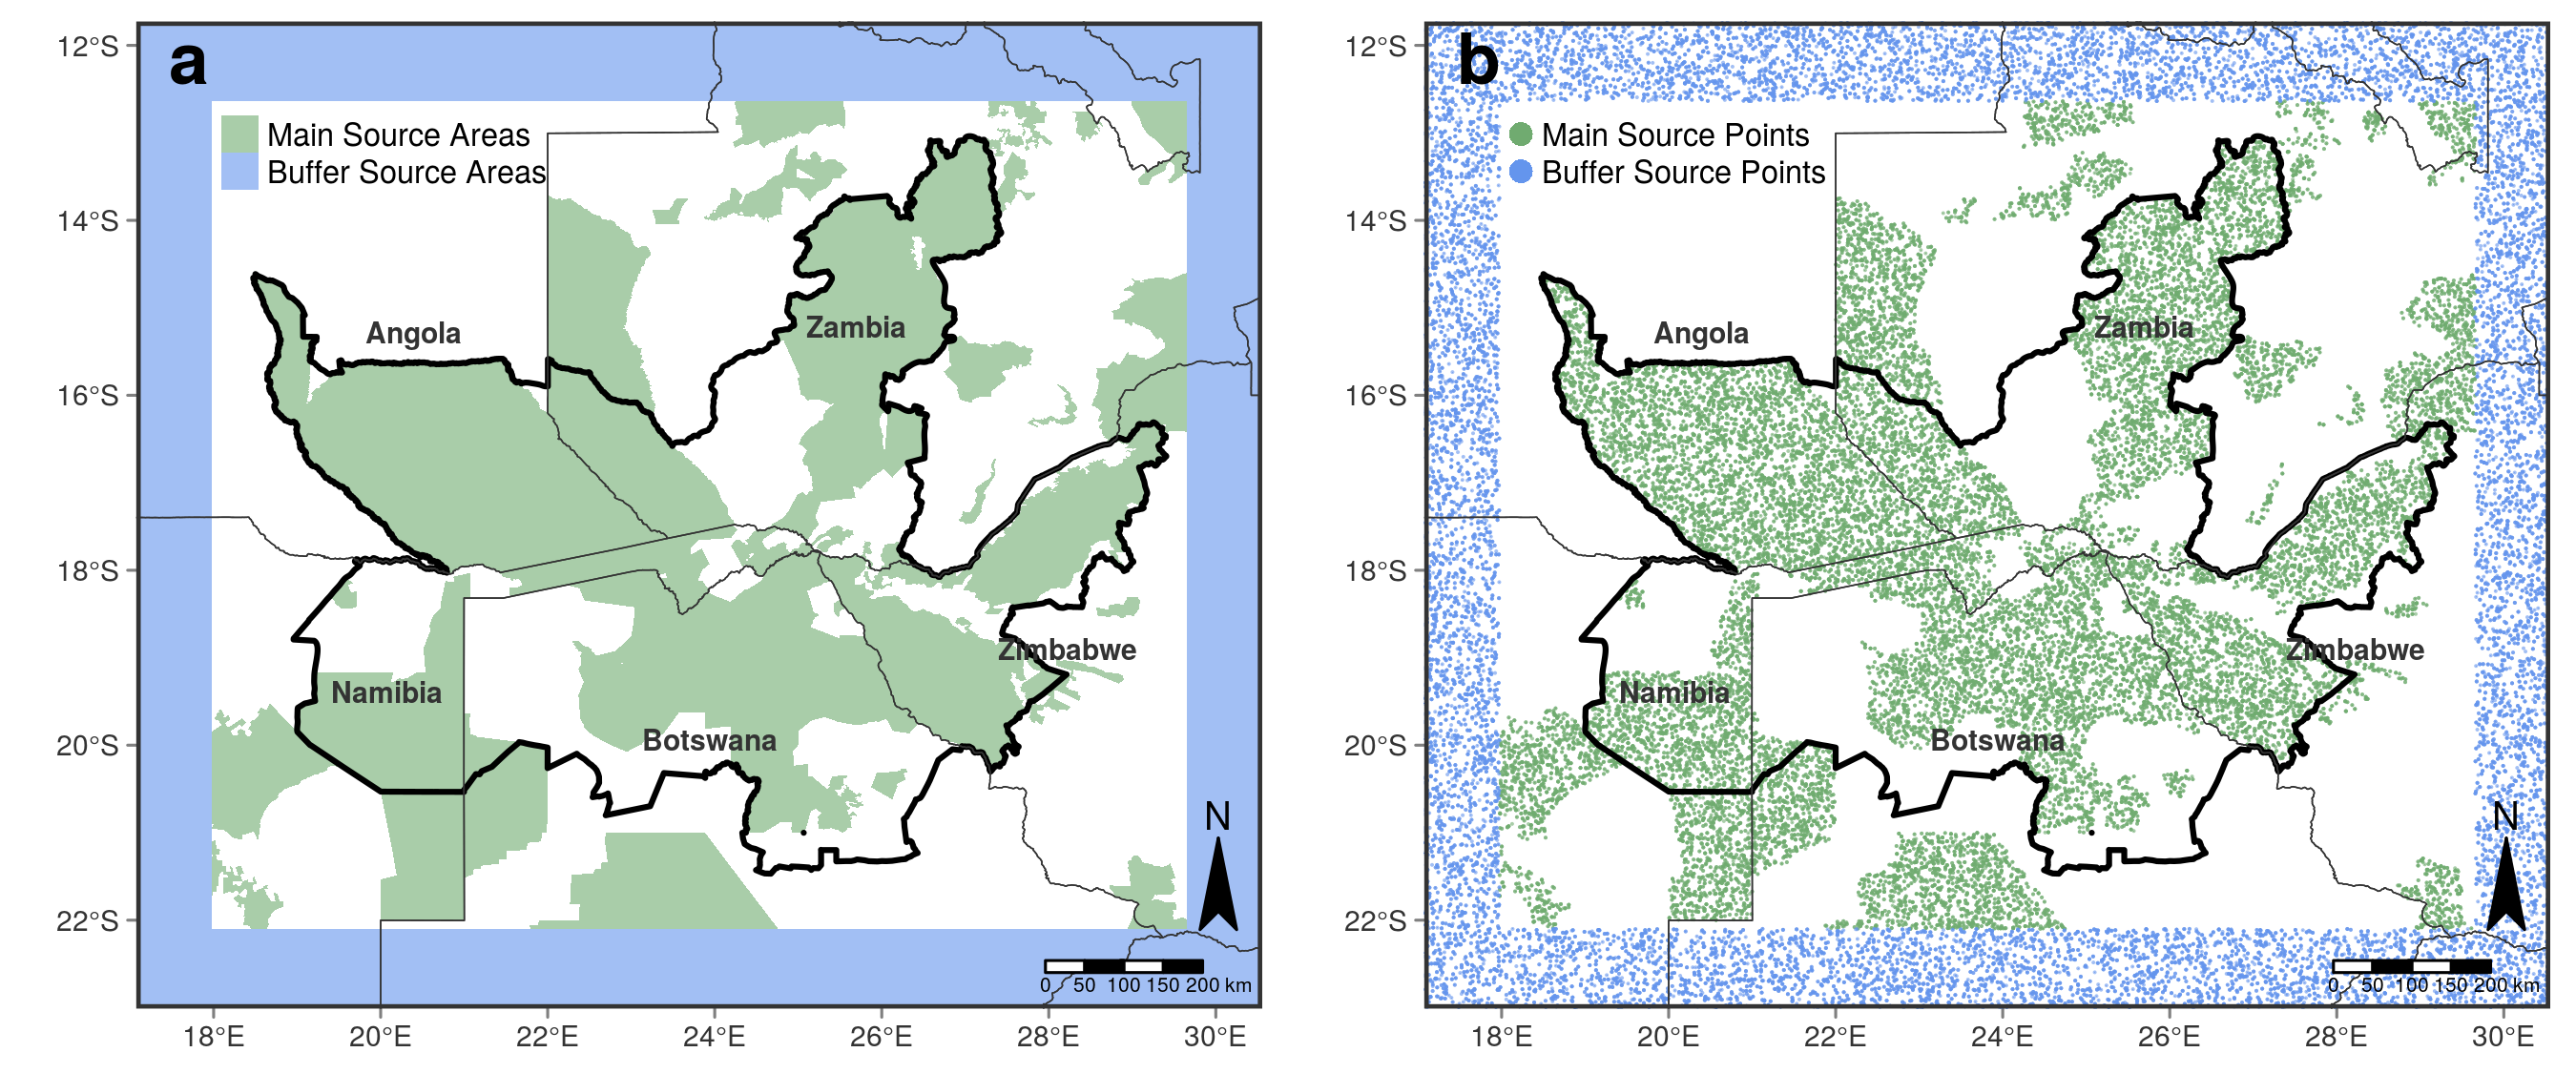
\includegraphics[width = \textwidth]{99_SourceAreas.png}
    \caption{(a) Different source areas from which we released virtual
    dispersers. We only considered contiguous protected areas (national parks,
    game reserves, and forest reserves) that were larger than 700
    km\textsuperscript{2} (green). This area corresponds to the average home
    range requirement for viable wild dog populations \citep{Pomilia.2015}. To
    render potential immigrants into the study system, we also initiated
    dispersers within a buffer zone (blue) surrounding the main study area. (b)
    Source points from which dipsersers were released. 50'000 dispersers were
    released from the main study area (green dots) and another 30'000 dispersers
    within the virtual buffer (blue dots).}
    \label{SourcePoints}
  \end{center}
\end{figure}

\subsection{Convergence (80\%)}
To verify that the number of simulated individuals sufficed to ensure reliable
estimates of connectivity, we evaluated how the relative traversal frequency
across the landscape changed as we increased the number of simulated
individuals. For this, we distributed 1'000 rectangular ``checkpoints'', each
with an extent of 5 km x 5 km at random locations inside the main study area. We
then determined the relative traversal frequency by simulated trajectories
through each checkpoint for different numbers of simulations (1 to 50'000). To
assess variability in the relative traversal frequency, we repeatedly sampled
trajectories 100 times and computed the mean traversal frequency across
replicates, as well as the 95\% prediction-interval. We deemed that a checkpoint
converged as soon as the width of the prediction interval for the traversal
frequency across replicates dropped below a value of 0.01.

\subsection{Heatmap (100\%)}
To identify dispersal hotspots across our study area, we created a heatmap
indicating the absolute frequency at which each raster-cell in the study area
was visited by virtual dispersers \citep{Hauenstein.2019, Peer.2008}. For this,
we rasterized all simulated trajectories and tallied them into a single map. If
the same trajectory crossed a raster-cell twice, we only counted it once,
thereby mitigating potential biases caused by individuals that were trapped and
moved in circles. To achieve high performance rasterization, we used the
R-package {\tt terra} \citep{Hijmans.2020}.

\subsection{Betweenness (80\%)}
To pinpoint areas of exceptional relevance for connecting remote regions inside
our study area, we converted simulated trajectories into a network and
calculated betweenness scores \citep{BastilleRousseau.2018}. For this, we
overlaid the study area (including the buffer) with a regular raster resolved at
5 x 5 km. The centerpoint of each raster-cell served as node in the final
network and we used the simulated trajectories to determine all transitions
occurring from one node to another, as well as the frequency at which those
transitions occurred. This resulted in an edge-list that we translated into a
weighted network using the r-package {\tt igraph} \citep{Gabor.2006}. Because
{\tt igraph} handles edge weights (\(\omega\)) as costs, we inverted the
traversal frequency in each cell by applying \(\omega = \frac{\sum_i^n{Traversal
Frequency_i}/n}{Traversal Frequency_i}\). Consequently, edges that were
traversed frequently were assigned low costs. Finally, we used the weighted
network to calculate the betweenness score of each raster-cell. Betweenness
measures how often a specific raster-cell lies on a shortest path between two
other raster-cells and is therefore a useful metric to detect movement corridors
\citep{BastilleRousseau.2018}.

\subsection{Inter-Patch Connectivity (80\%)}
We assessed inter-patch connectivity between national parks located in our study
area to examine functional links between distinct patches in the KAZA-TFCA. The
decision to focus on national parks was purely out of simplicity and does not
imply that connections between other regions are impossible. In fact, the same
logic could easily be expanded to include other protected areas. To quantify
inter-patch connectivity, we computed the relative frequency at which dispersers
originating from one national park successfully moved into another national
park. Successful movement was said to be achieved if the individuals' trajectory
intersected with the corresponding national park at least once. We also recorded
the number of steps required until the first intersection with the polygon of
the respective national park. This allowed us to determine \textit{if} and
\textit{how often} dispersers moved between certain national parks, as well as
\textit{how long} dispersers had to move to realize those connections.

\section{Results}
\subsection{Movement Model (80\%)}
Compared to the base model reported in \citep{Hofmann.2021}, our most
parsimonious movement model retained several additional interactions between
habitat covariates and movement covariates (\Cref{MovementModel} and
\Cref{MovementModelNumbers}). Although several models received an AIC weight
above zero (Table 1 in Appendix S1), we only considered results from the most
parsimonious model for simplicity. All models with positive AIC weight included
similar covariates (Table S1), so this decision only marginally influenced
subsequent analyses. Plots that aid with the interpretation of the final model
are provided in Appendix S2.

Assuming that all other covariates are held constant at their means, the habitat
kernel reveals that dispersing wild dogs avoid water but prefer its proximity.
Similarly, dispersers avoid areas that are covered by woodlands, yet prefer
regions covered by shrublands or grasslands. Finally, dispersers avoid movement
through landscapes that are dominated by humans. Effect sizes are strong and,
except for effect of \textsf{distance to water}, statistically clear on the 5\%
significance level.

With regards to the movement kernel, the positive estimate for \textsf{cos(ta)}
indicates that dispersers move with directional persistence, unlike what was
proposed by the uniform turning angle distribution. Moreover, directionality is
particularly pronounced when dispersers realize large steps (move quickly), as
indicated by the positive estimates for \textsf{cos(ta):sl} and
\textsf{cos(ta):log(sl)}. Finally, the negative estimate for the interaction
\textsf{sl:LowActivity} reveals that wild dogs realize shorter steps (move
slower) outside the main activity periods (during sunrise and sunset). Aside
from the interaction \textsf{sl:LowActivity}, which appears to strongly
influence movmement behavior, effect sizes are moderate, but mostly significant
on the 5\% significance level.

When looking at the interactions between movement and habitat kernels, we
observe that movement behavior is contingent on habitat conditions. For example,
there's strong evidence that dispersers realize smaller steps in areas covered
by water or areas covered by wooldand, yet it appears that steps are larger in
regions dominated by shrubs/grassland, and shorter when the distance to water is
high. Correspondingly, the model suggests that directionality is lower in areas
dominated by humans but more pronounced when dispersers are far from water.
However, except for the effect of \textsf{sl:Water}, effect sizes and
statistical significance are moderate.

The k-fold cross-validation procedure reveals that our model substantially
outperforms a random guess (\Cref{MovementModel}b) and therefore correctly
assigns a high selection score to realized steps. Confidence intervals of
\(\bar{r}_{s, realized}\) and \(\bar{r}_{s, random}\) do not overlap and
therefore proof a reliable prediction. Furthermore, the significant correlation
between ranks and corresponding frequencies for realized steps indicates a good
fit between predictions and observations (\Cref{MovementModel}b). In comparison
to the base model (\(\bar{r}_{s, realized} = -0.55\); \citealp{Hofmann.2021}),
the inclusion of interactions between movement and habitat covariates slightly
improved model performance.

\begin{figure}
  \begin{center}
    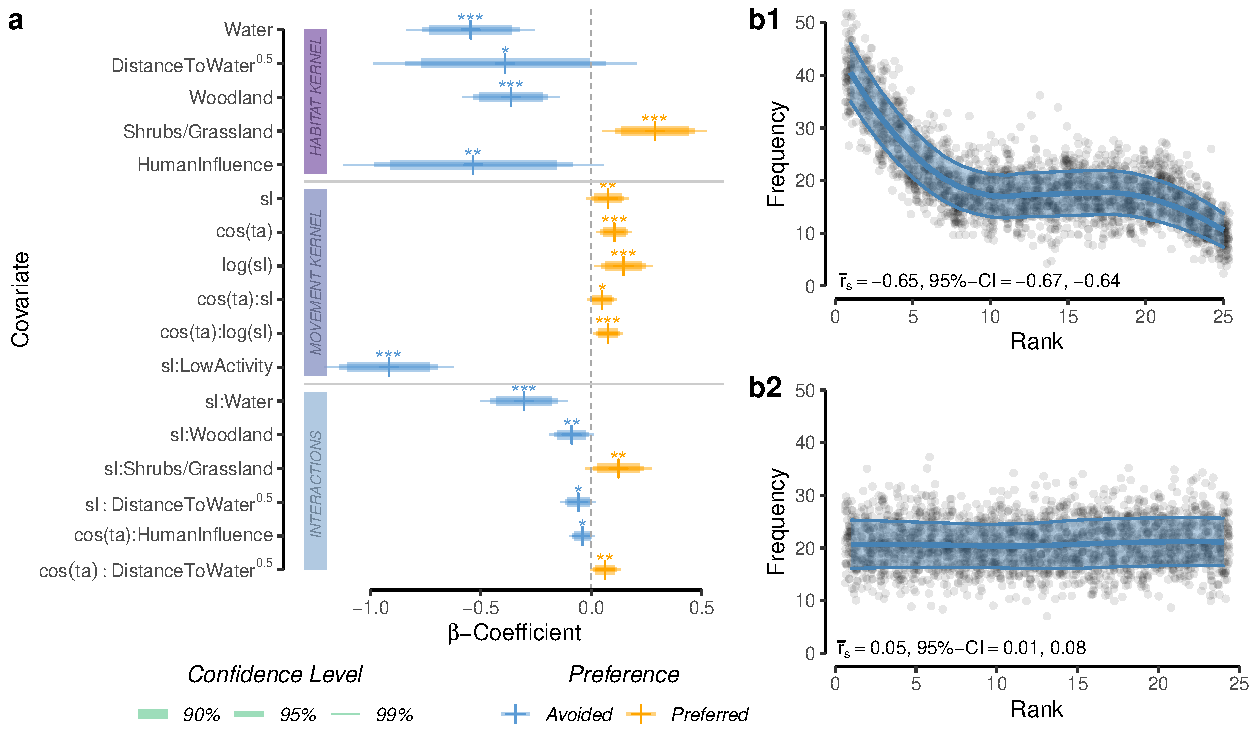
\includegraphics[width=\textwidth]{99_MovementModel}
    \caption{(a) Most parsimonious movement model for dispersing wild dogs. The
    model includes a habitat kernel, a movement kernel, as well as their
    interactions. The horizontal line segments delineate the 90\%, 95\%, and
    99\% Confidence-Intervals for the respective \(\beta\)-coefficients.
    Significance codes: * \(p < 0.10\), ** \(p < 0.05\), *** \(p < 0.01\). (b)
    Results from the k-fold cross validation procedure. The upper plot shows
    rank frequencies of realized steps according to model predictions with known
    preferences, whereas the lower plot shows rank frequencies of realized steps
    when assuming random preferences. The blue ribbon shows the prediction
    interval around a loess smoothing regression that we fitted to ease the
    interpretation of the plots. The significant correlation between rank and
    associated frequency in (b1) highlights that the most parsimonious model
    successfully outperforms a random guess (b2) and assigns comparably high
    selection scores to realized steps.}
    \label{MovementModel}
  \end{center}
\end{figure}

\begin{table}
  \begin{center}
  \caption{Most parsimonious movement model for dispersing wild dogs. The model
  consists of a movement kernel, a habitat kernel, and their interactions. The
  movement kernel describes preferences with regards to movement behavior,
  whereas the habitat kernel describes preferences with respect to habitat
  conditions. Interactions between the two kernels indicate that movement
  preferences are contingent on habitat conditions. Note that all covariates
  were standardized to a mean of zero and standard deviation of 1. Plots to aid
  with the interpretation of this model are given in Appendix S2.}
  \label{MovementModelNumbers}
  \resizebox{\textwidth}{!} {
    \begin{threeparttable}
      \begin{tabular}{llrrrc}
        \toprule
        Kernel & Covariate & Coefficient & SE & p-value & Sign. \\
        \midrule
        \multirow{5}{*}{Habitat Kernel}
         & Water & -0.546 & 0.112 & \(<\) 0.001 & *** \\
         & DistanceToWater \textsuperscript{0.5} & -0.390 & 0.231 & 0.092 & * \\
         & Woodland & -0.364 & 0.086 & \(<\) 0.001 & *** \\
         & Shrubs/Grassland & 0.288 & 0.092 & 0.002 & *** \\
         & HumanInfluence & -0.535 & 0.229 & 0.019 & ** \\
        \hdashline
        \multirow{6}{*}{Movement Kernel}
         & sl & 0.075 & 0.037 & 0.042 & ** \\
         & cos(ta) & 0.105 & 0.031 & 0.001 & *** \\
         & log(sl) & 0.146 & 0.051 & 0.004 & *** \\
         & cos(ta) : sl & 0.049 & 0.026 & 0.064 & * \\
         & cos(ta) : log(sl) & 0.076 & 0.026 & 0.003 & *** \\
         & sl : LowActivity & -0.917 & 0.113 & \(<\) 0.001 & *** \\
        \hdashline
        \multirow{5}{*}{Interactions}
         & sl : Water & -0.305 & 0.076 & \(<\) 0.001 & *** \\
         & sl : Woodland & -0.089 & 0.039 & 0.023 & ** \\
         & sl : Shrubs/Grassland & 0.124 & 0.058 & 0.032 & ** \\
         & sl : DistanceToWater \textsuperscript{0.5} & -0.058 & 0.031 & 0.056 & * \\
         & cos(ta) : HumanInfluence & -0.040 & 0.022 & 0.070 & * \\
         & cos(ta) : DistanceToWater \textsuperscript{0.5} & 0.063 & 0.026 & 0.017 & ** \\
         \bottomrule
      \end{tabular}
       \begin{tablenotes}
         \item \textit{Significance codes: * \(p < 0.10\) \quad ** \(p < 0.05\)
         \quad *** \(p < 0.01\)}
       \end{tablenotes}
    \end{threeparttable}
    }
  \end{center}
\end{table}

\subsection{Dispersal Simulation (80\%)}
On a machine with an octacore AMD Ryzen 7 2700X processor (8 x 3.6 GHz) and 64
GB of RAM, a batch of 1'000 simulated dispersers moving over 2'000 steps
required 90 minutes to compute (\(\mu = 88.90\), \(\sigma = 1.87\)).
Consequently, the simulation of all 80'000 dispersers (160 Mio. steps)
terminated after 120 hours (i.e. five days). Comparable simulations will be
substantially faster for smaller study areas and lower resolution covariates, as
the covariate extraction from large and high-resolution rasters was
computationally the most demanding task. Out of the 50'000 dispersers initiated
inside the main source area \Cref{SourcePoints}(a), only 4.5\% eventually hit a
map boundary, suggesting that we successfully prevented biases due to boundary
effects. In contrast, 78\% of the 30'000 dispersers originating from the buffer
zone eventually hit a map boundary, yet this was to be expected since many of
those dispersers originated from source points located close to the map
boundary.

\subsection{Convergence (80\%)}
Our examination of the traversal frequency as a function of the number of
simulated dispersers shows that the mean traversal frequency stabilizes already
after very few simulations and changes only little when adding further
dispersers (\Cref{Convergence} (a) and (b)). While variability keeps decreasing
with additional dispersers, the marginal benefit of adding further dispersers
steeply decreases with a negative-exponential trend (\Cref{Convergence} (c)).

\begin{figure}
  \begin{center}
    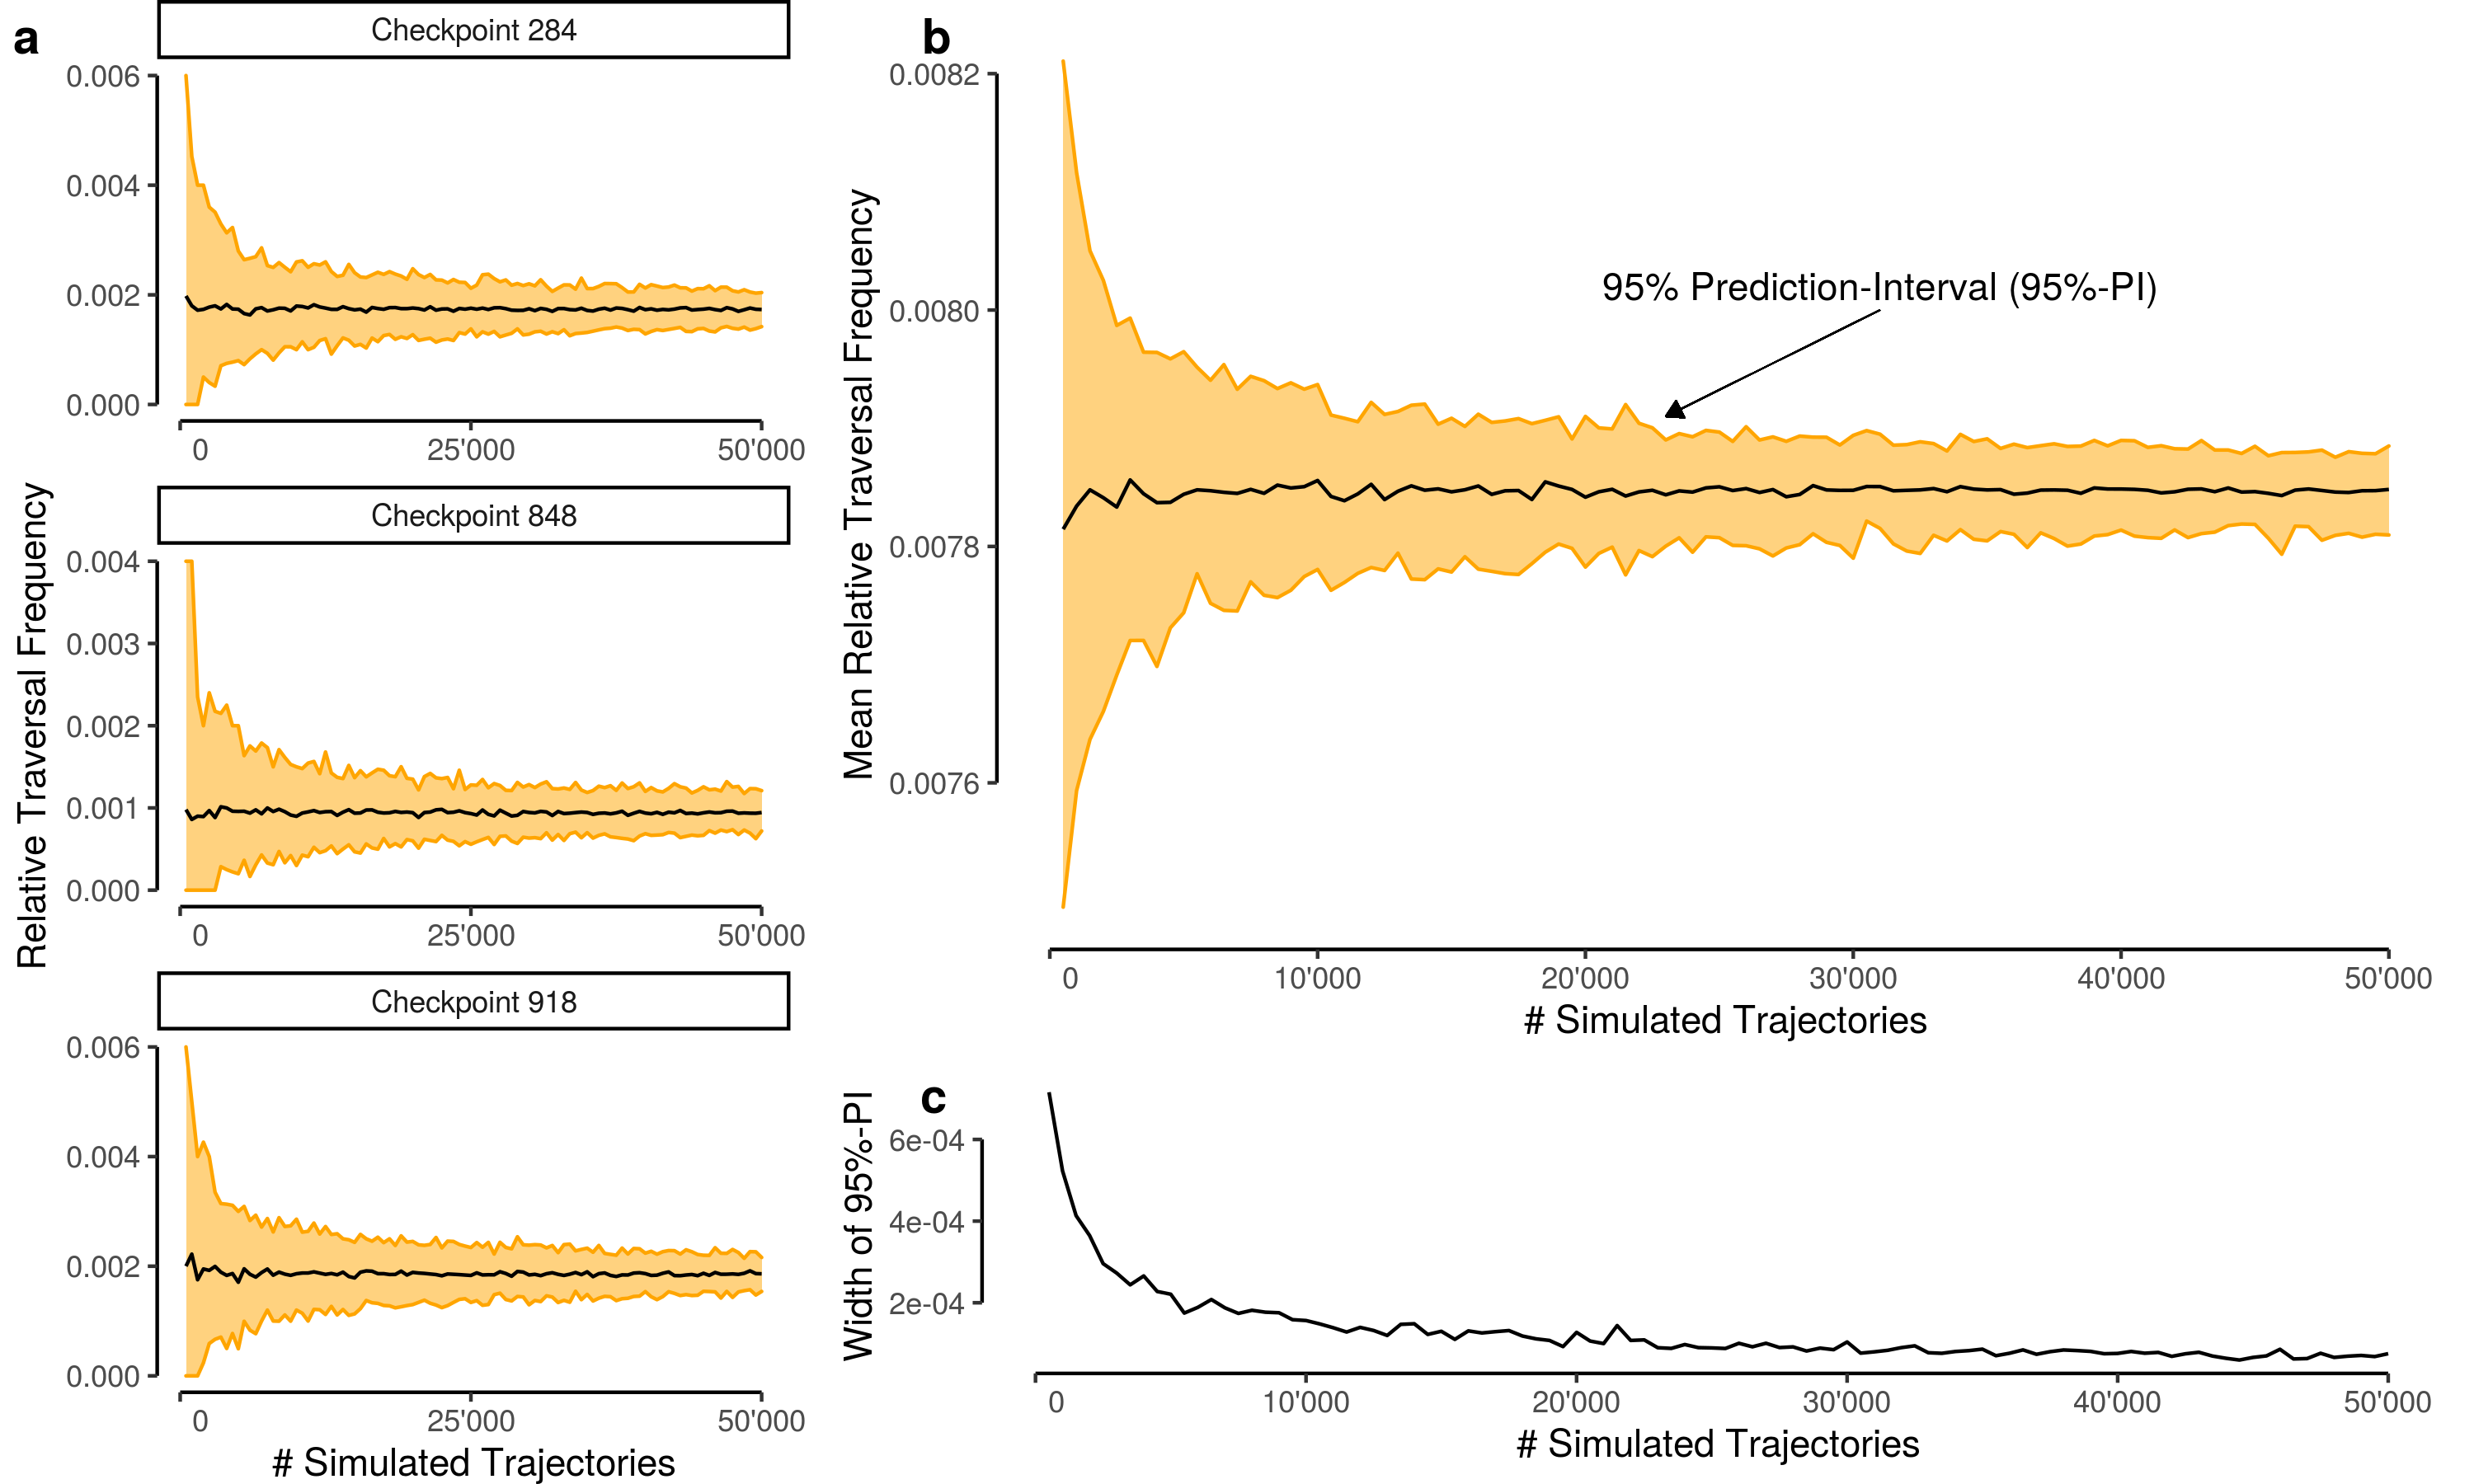
\includegraphics[width=\textwidth]{99_Convergence}
    \caption{Relative traversal frequency through 1'000 checkpoints (5 km x 5)
    distributed randomly across the study area. The relative traversal frequency
    is plotted against the number of simulated individuals to visualize how
    quickly the metric converges to a steady state. (a) Replicated (100 times)
    relative traversal frequencies across three randomly chosen checkpoints as
    well as the corresponding 95\% prediction interval (PI). (b) Averaged
    relative traversal frequency across all checkpoints and replicates including
    a 95\% PI. (c) Width of the PI in relation to the number of simulated
    dispersers.}
    \label{Convergence}
  \end{center}
\end{figure}

\subsection{Heatmap (80\%)}
\Cref{Heatmap} depicts the heatmap of all 80'000 simulated trajectories
resulting after 2'000 steps. The map shows that large portions of land beyond
the borders of the KAZA-TFCA are only infrequently visited by dispersers (dark
blue areas), whereas within the KAZA-TFCA several extensive regions are
regularly traversed (bright yellow and red areas). Most notably, the region in
northern Botswana south of the Linyanti swamp stands out as highly frequented
dispersal hotspot. Still, the presence of several massive water bodies, such as
the Okavango Delta, the Makgadikgadi Pan, and the Linyanti swamp, poses
considerable dispersal barriers that limit realized connectivity within the
KAZA-TFCA. Similarly, dispersal across Zambia's and Zimbabwe's part of the
KAZA-TFCA appears to be limited, as only few areas are successfully traversed by
dispersers. This can largely be attributed to substantial human influences
resulting from high human density, roads, and agricultural activities in these
areas. Outside the KAZA-TFCA, the most heavily used regions include the areas
inside the Central Kalahari National Park in Botswana, the area south-west of
the Khaudum National Park in Namibia, and the area around the Liuwa Plains
National Park in Zambia.

\begin{figure}
  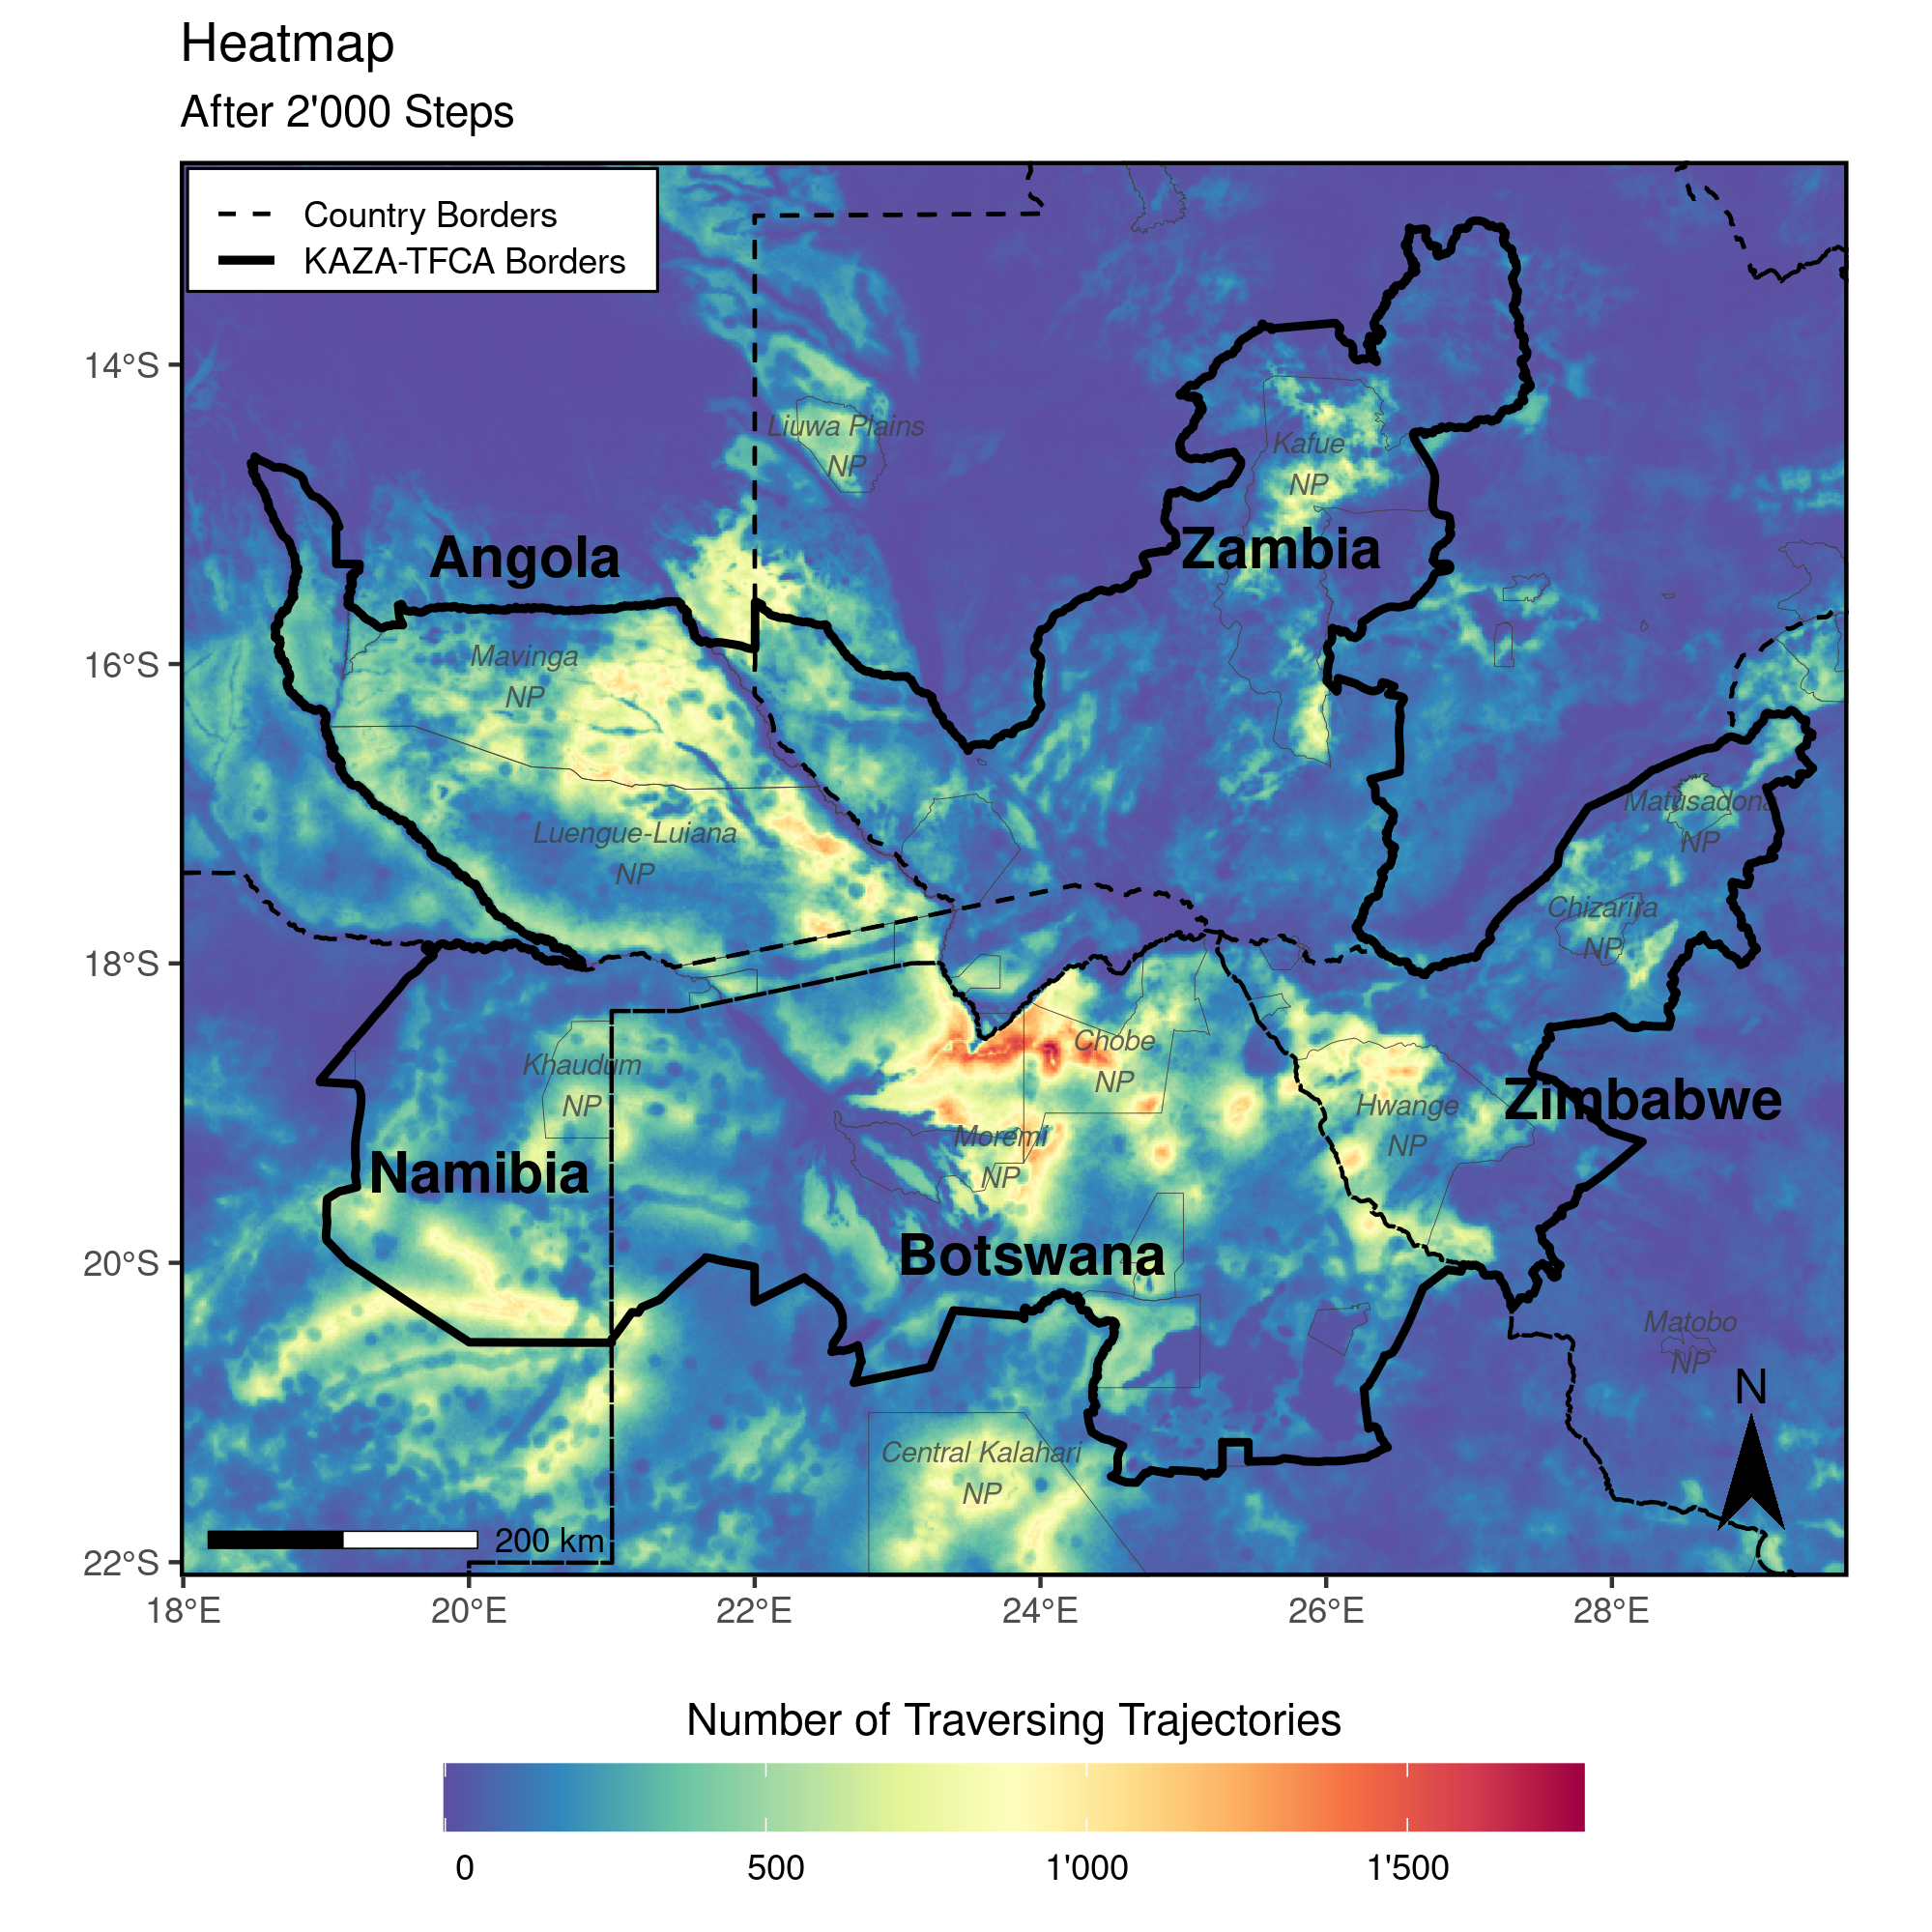
\includegraphics[width=\textwidth]{99_Heatmap.png}
  \caption{Heatmap showing traversal frequencies of 80'000 simulated dispersers
  moving 2'000 steps across the KAZA-TFCA. Simulations were based on an
  integrated step selection model that we fit to the movement data of dispersing
  African wild dogs. To generate the heatmap, we rasterized and tallied all
  simulated trajectories. Consequently, the map highlights areas that are
  frequently traversed by virtual dispersers. Additional heatmaps showing the
  traversal frequency for different numbers of simulated steps are provided in
  Appendix S3.}
  \label{Heatmap}
\end{figure}

\subsection{Betweenness (80\%)}
Betweenness scores after 2'000 simulated steps are presented in
\Cref{Betweenness} and reveal a set of discrete dispersal corridors. Again, the
region in northern Botswana stands out as crucial dispersal hub that connects
more remote regions in the study system. Towards east, the extension of this
corridor runs through the Chobe National Park into the Hwange national park.
From there, a further extension connects to the distant Matusadona National Park
in Zimbabwe. Northwest of the Linyanty ecosystem, a major corridor expands into
Angola, where it splits and finally traverses over a long stretch of unprotected
area into the Kafue National Park in Zambia. Several additional corridors with
slightly lower betweenness scores exist, yet most of them run within the
boundaries of the KAZA-TFCA. In general, only few corridors directly link the
peripheral regions of the KAZA-TFCA. For instance, there are only few corridors
between the Matusadona National Park in Zimbabwe and the Kafue National Park in
Zimbabwe. Similarly, there are no direct links between the Zimbabwean and
Angolan ``spikes'' of the KAZA-TFCA.

\begin{figure}
  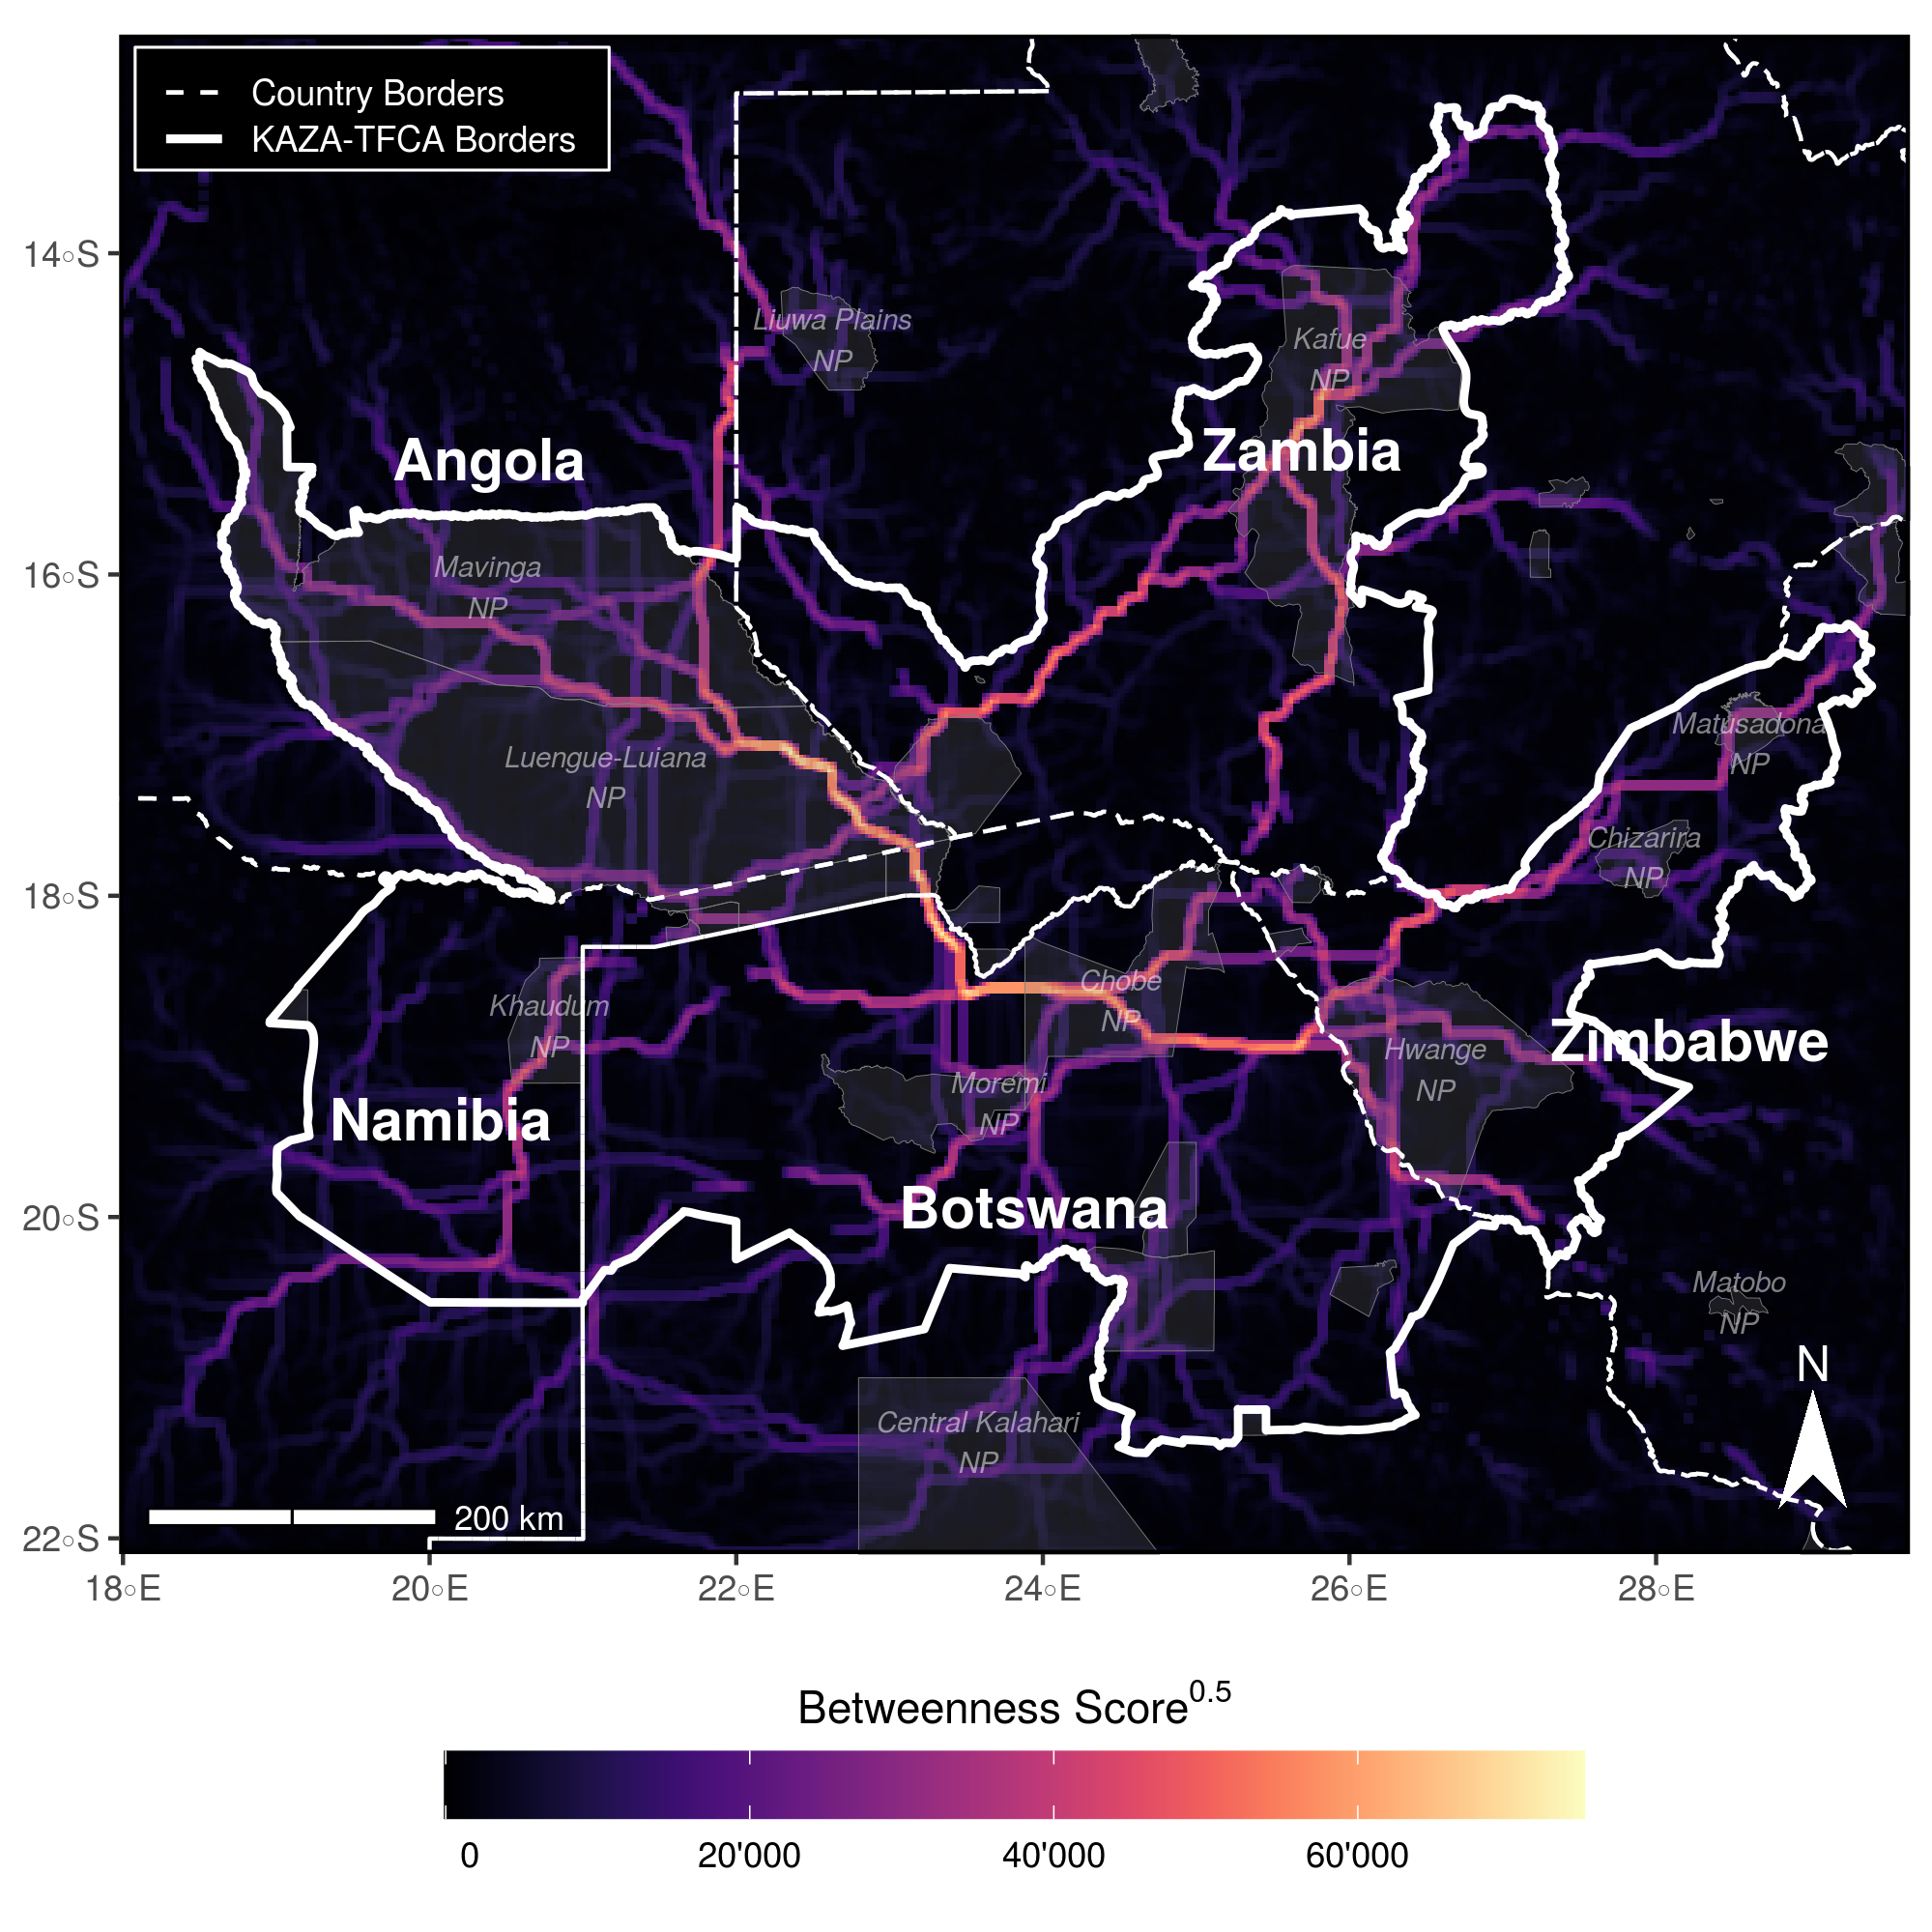
\includegraphics[width=\textwidth]{99_Betweenness.png}
  \caption{Map of betweenness scores, highlighting distinct dispersal corridors
  and potential bottlenecks. A high betweenness score indicates that the
  respective cells are exceptionally relevant in connecting different regions in
  the study area. That is, the higher the betweenness score, the more often a
  pixel lies on a shortest path between adjacent areas. In this sense the metric
  can be used to pinpoint discrete movement corridors. Note that we
  square-rooted betweenness scores to improve visibility of corrdiors with low
  scores. Betweenness scores were determined by converting simulated dispersal
  trajectories into a large network. Note that we square-rooted betweenness
  scores to improve the visibility of corridors with low betweenness scores.}
  \label{Betweenness}
\end{figure}

\subsection{Inter-Patch Connectivity (80\%)}
Results from the analysis of inter-patch connectivity are given in
\Cref{AreasReached}. The figure shows all realized links by simulated dispersers
between national parks and indicates the average duration a disperser had to
move to realize those links. It is again worth pointing out that the figure is
only intended as an example, as for clarity we only considered connectivity
between national parks (NPs), albeit plenty of links between other protected
areas exist. As can be seen from the number, thickness, and color of arrows,
inter-patch connectivity between NPs in Angola, Namibia, and Botswana is
comparably high and dispersal events between those areas short. In contrast, we
see that connections into the Kafue NP in Zambia require more steps and are
fewer in general. Similarly, there is a lack of connections into Zimbabwe's
Chizarira and Matusadona NP and the more distant Lower Zambezi and Mana Pools
NPs. In some cases, one can also detect imbalances between ingoing and outgoing
links, hinting at potential source-sink dynamics that occur due to asymmetries
in landscape permeability depending on the origin. For instance, while a large
portion of dispersers from the Chizaria NP in Zimbabwe manage to move into the
Hwange NP, there are comparably few dispersers that succeed in the opposite
direction.

% The map shows all realized links by simulated dispersers between national parks
% and indicates the average duration a disperser had to move to realize those
% links. For instance, 6.8 \% of the simulated dispersers originating from the
% Moremi National Park successfully reached the Chobe National Park and 4.2 \% the
% Hwange National Park in Zimbabwe. On average, dispersers moved for 623 steps
% before arriving at Chobe (SD = 520) and for 1'413 steps before arriving at
% Hwange (SD = 371). While the map only depicts connections between national
% parks, this does not imply that no connections to other protected areas exist
% and is the result of our simplifying assumptions above. Interestingly, while we
% identified a potential dispersal corridor between Angola's NPs and the Kafue NP
% in Zambia, \Cref{AreasReached} suggests that this link is only rarely realized
% and requires very long dispersal events. In contrast, we find that dispersal
% between the Moremi NP and Chobe NP are relatively frequent and require fewer
% steps, which can be expected given that the areas are located close to each
% other.

\begin{figure}
  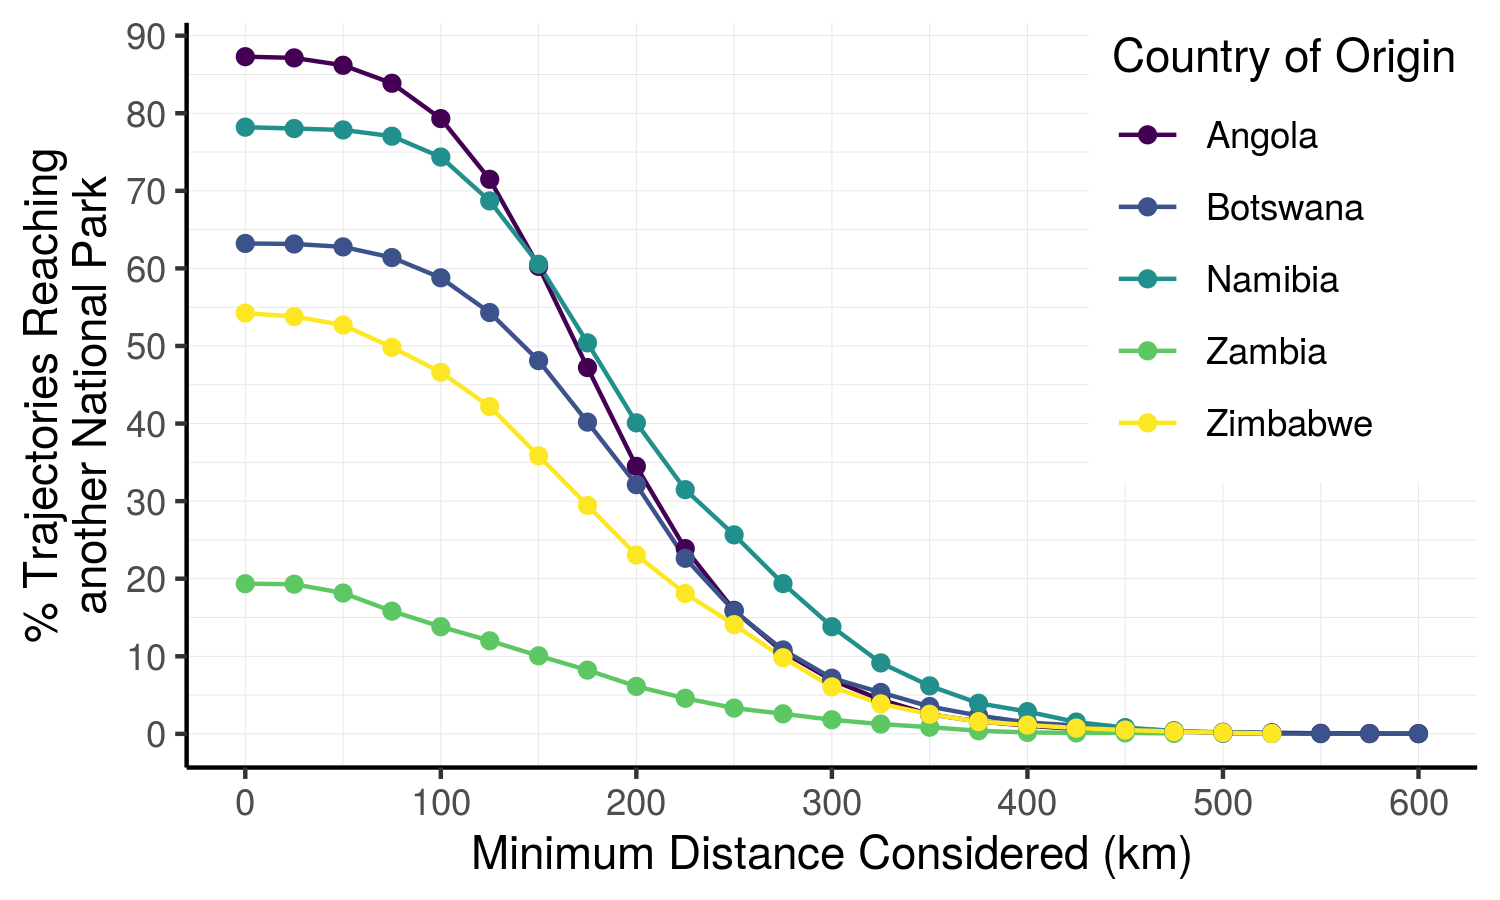
\includegraphics[width=\textwidth]{99_AreasReached.png}
  \caption{Network on simulated dispersal trajectories highlighting connections
  between national parks (dark green). Yellow bubbles represent the center of
  the different national parks and are sized in relation to the number of
  simulated dispersers originating from each park. Black dots represent national
  parks that were smaller than 700 km\textsuperscript{2} and therefore did not
  serve as source areas. Arrows between national parks illustrate between which
  national parks the simulated dispersers successfully moved and the color of
  each arrow shows the average number of steps (4-hourly movements) that were
  necessary to realize those connections. Additionally, the line thickness
  indicates the relative number of dispersers originating from a national park
  that realized those connections. Note that a similar network view could be
  adopted to investigate connectivity between other protected areas need not to
  be restricted to national parks.}
  \label{AreasReached}
\end{figure}

\section{Discussion}

% Short Summary
\subsection{Short Summary (90\%)}
We used ISSFs to analyse data of dispersing wild dogs and to parametrize a fully
mechanistic movement model describing how dispersers move through the available
landscape. We employed the parametrized model as an individual-based movement
model to simulate 80'000 dispersing wild dogs moving 2'000 steps across the
extent of the KAZA-TFCA, the world's largest transboundary conservation area.
Based on simulated dispersal trajectories, we derived three complementary maps,
each geared towards a better understanding of dispersal and landscape
connectivity. The set of maps included a heatmap, revealing frequently traversed
areas, a betweenness-map, delineating critical dispersal corridors, and a map of
inter-patch connectivity, indicating the presence or absence of functional links
between national parks as well as the average dispersal duration required to
realize those links. We thereby showcase that ISSFs offer a simple, yet powerful
framework to parametrize movement models and simulate dispersal to assess
landscape connectivity. Importantly, individual-based simulations from ISSFs
overcome several conceptual shortcomings inherent to more traditional
connectivity modeling techniques, such as least-cost path analysis and circuit
theory.

% Movement Model
\subsection{Movement Model (80 \%)}
Our movement model of dispersing wild dogs comprised a habitat kernel, a
movement kernel, and their interactions. Thus, the model rendered habitat and
movement preferences of dispersers, as well as how their movement preferences
were affected by habitat conditions. Parameter estimates from the habitat kernel
revealed that dispersers avoid water, prefer its proximity, avoid woodland,
prefer shrubs/grassland, and avoid areas dominated by humans. These results are
consistent with findings from previous studies on dispersing wild dogs
\citep{DaviesMostert.2012, Masenga.2016, Woodroffe.2019, Oneill.2020}, as well
as with a base model that we developed focussing on dispersing wild dogs'
habitat kernel \citep{Hofmann.2021}.

By expanding the base model by a proper movement kernel, we were able to model
several additional complexities inherent to dispersal. For instance, it is well
known that dispersers usually move with directional persistence
\citep{Cozzi.2018, Hofmann.2021} and that step lengths are typically correlated
with turning angles \citep{Morales.2004, Borger.2012}. That is, larger steps
usually coincide with smaller turning angles and vice versa. While such behavior
could be captured by jointly sampling turning angles and step lengths from
copula probability distributions \citep{Hodel.2021}, the ISSF framework allowed
us to model similar behavior directly using the movement model. Besides
accounting for directional persistence and correlations between step lengths and
turning angles, we also allowed for interactions that rendered the fact that
wild dogs mainly move during the darker morning and evening hours, whereas they
tend to rest during the remainder of the day.

By allowing interactions between habitat covariates and movement covariates, we
furthermore accounted for the fact that movement and habitat preferences are
interdependent. For example, the final model retained an interaction between
water cover and step length, showing that dispersers are more likely to realize
short steps (i.e. move slower) in areas covered by water and large steps in
areas located on dryland. Likewise, the parameter estimate for the interaction
between water cover and turning angles revealed that dispersers move less
directional across water bodies than across dryland. We believe that this is
owed to the fact that wild dogs wade or swim when traversing waterbodies, thus
resulting in slower, more tortuous movements. Besides this, our model also
suggested that dipsersers preferably realize shorter steps when moving through
woodland, but larger steps when moving across shrubs/grassland. This can likely
be linked to wild dogs' resting behavior, as wild dogs usually use open areas to
quickly move over long distances \citep{Abrahms.2017} but seek shade and
protection below the woodland canopy when resting \citep{Creel.2002}.

\subsection{Simulation (80\%)}
Based on the above described movement model, we simulated 80'000 dispersers
moving 2'000 steps across the landscapes of the KAZA-TFCA. On a modern desktop
machine, this simulation required five days of computation. The long simulation
time was primarily caused by the massive extent considered (ca. 1.8 Mio. km
\textsuperscript{2} when including the buffer) and the large number of
dispersers simulated. Most connectivity studies are limited to much smaller
extents (e.g. \citealp{Kanagaraj.2013, Clark.2015, McClure.2016, Abrahms.2017,
Zeller.2020}) and will therefore achieve faster simulation times. We also
believe that fewer simulated dispersers will often suffice, as the relative
traversal frequency by simulated individuals through randomly placed checkpoints
in the study area converged already after 10'500 simulated individuals in our
case. The required number of simulated individuals will, however, vary depending
on the structure of the landscape and the dispersal ability of the focal
species.

\subsection{Maps (70\%)}
The heatmap resulting from our dispersal simulation highlighted that a large
portion of simulated dispersers traversed the Moremi NP and the Chobe NP in
northern Botswana. We already recognized the same area as dispersal hotspot
using least-cost path and least-cost corridor analysis \citep{Hofmann.2021}, yet
some researchers questioned whether this was just the logical consequence of the
region being in the center of the study area and least-costly routes being
enforced between pre-defined start and endpoints. Using least-cost approaches,
this claim is difficult to disprove, as all identified routes have to completely
run within the study area and will always be enforced between a start and
endpoint. With our simulation, on the other hand, dispersers were able to leave
the study area and were not enforced to move towards a known endpoint. Despite
this, a majority of simulated individuals traversed the central region in
northern Botsana, so we conclude that this dispersal hotspot is not caused by
geometric properties but results from landscape characteristics and the location
of source areas.

Overall, the heatmap gives a good overview of the intensity of use in different
areas, yet it is not well suited for pinpointing discrete movement corridors,
which is why we also computed a betweenness-map. In contrast to the heatmap, the
betweenness-map puts stronger emphasis on areas that are used as stepping stones
into other regions of the study area and thereby highlights discrete dispersal
corridors or bottlenecks \citep{BastilleRousseau.2018}. Interestingly, the
central region in northern Botswana again stands out, implying that the region
is not only frequently visited, but also promotes the relocation of individuals
into more remote regions of the KAZA-TFCA. While this is an example of an area
were both the traversal frequency \textit{and} the betweeness score is high,
there are other instances where only one of the metrics is pronounced. For
example, while the area between the Lengue-Luiana NP in Angola and the Kafue NP
in Zambia receives a high betweenness-score, we find that the same area is only
rarely traversed by dispersers according to the heatmap. Consequently, despite
the region's importance for linking Angola's NPs to Zambia's NP, only few
simulated dispersers actually manage to successfully traversed it. Conversely,
while the area inside the Central Kalahri NP is traversed by many dispersers,
the betweenness map indicates that the same region does not serve as major
stepping stone into other regions of the study area.

To complete the picture, we also computed inter-patch connectivity between NPs,
highlighting functional links and expected dispersal durations between each
national park in the study area. The map showed that movements from Angola into
Zambia's Kafue NP are not only rare, but they also require many steps until they
are realized. Conversely, we find that dispersal between the Moremi NP and Chobe
NP are relatively frequent and require fewer steps, which can be expected given
that the areas are located close to each other.

Together, these examples nicely illustrate how powerful a combination of
different connectivity metrics can be in deepening our understanding of
landscape connectivity. Each map that we produced from simulated trajectories
accentuated a different aspect of connectivity, together providing a
comprehensive view on dispersal and landscape connectivity. The heatmap, for
example, put emphasis on areas where movement is concentrated, regardless
whether such areas truly contribute to geneflow or whether they represent ``dead
ends'' that do not connect distinct patches. The betweenness map, on the other
hand, pronounced those areas that are relevant in connecting different regions
in the landscape and highlights potential bottlenecks. Finally, the map of
inter-patch connectivity illustrated the frequency at which dispersal between
distinct patches occurs, as well as the average dispersal duration required for
individuals to move between them.

% Other studies that use similar simulations
\subsection{Related Literature (80\%)}
Our approach of simulating movement to assess connectivity is closely related to
a series of previously published papers. \cite{Clark.2015}, for instance, fitted
a regular SSF to American black bears (\textit{Ursus americanus}) and employed
the estimated model parameters to simulate movement and identify the most likely
movement corridors between four habitat patches. For the same species,
\cite{Zeller.2020} used regular SSFs and forecasted seasonal habitat
connectivity under changing land-use. As both of these studies relied on
\textit{regular} SSFs, rather than \textit{integrated} SSFs, neither of them was
able to account the interdependence between habitat and movement preferences. As
such, movement behavior was assumed to be independent of habitat conditions. In
addition, both studies lacked data collected during dispersal and instead
employed data on residents to estimate connectivity. Although preferences during
residence and dispersal may coincide for some species \citep{Fattebert.2015},
there is compelling evidence suggesting that dispersers more readily cross areas
avoided by residents \citep{Elliot.2014, Gaston.2016, Abrahms.2017,
Keeley.2017}. The use of data collected during residence may therefore result in
biased model estimates that distort our view on connectivity, causing a
misallocation of scarce conservation funds \citep{Elliot.2014}. Another set of
related studies that uses simulations from (regular and integrated) SSFs has
been conducted by \cite{Potts.2013} and \cite{Signer.2017}, yet the primary
focus of these papers lied on the estimation of steady-state utilization
distributions and not the investigation of connectivity between habitat patches.

\subsection{Benefits \& Modeling Decisions with ISSF Simulations (70\%)}
% Does not enforce route towards known endpoint
A simulation-based approach as proposed in this article offers several
advantages over traditional connectivity modeling techniques such as LCPA or CT.
In contrast to LCPA, for instance, an individual-based simulation does not
require to assume known endpoints. Instead, each endpoint emerges naturally from
a simulated dispersal trajectory. The ability of not having to provide
pre-determined is particularly valuable for dispersal studies, because
dispersers often venture into unfamiliar territory and are therefore unlikely to
know the destination of their journey \citep{Elliot.2014, Abrahms.2017,
Cozzi.2020}. Moreover, LCPA always enforces a connection towards the predefined
endpoints, even if associated movement costs are unreasonably high. With
simulations from ISSFs this is no longer the case. A connectivity model that
does not require pre-defined endpoints also ensures that movement corridors are
not enforced between certain start- and endpoints, which permits to detect
potential routes that do not lead into suitable habitats but into ecological
traps \citep{Dwernychuk.1972, VanDerMeer.2014} or areas with a high
susceptibility for human wildlife conflicts \citep{Cushman.2018}.

% Explicit Representation of Time
In contrast to LCPA and CT, simulations from ISSFs furthermore yield the
advantage of an explicit representation of time. This enables to answer
questions such as: ``\textit{How long will it take a disperser to move from A to
B?}'' or ``\textit{Is it possible for a disperser to move from A to B within X
days?}'' These are important questions that shift the focus from a structural to
a more functional view on connectivity, which is usually desirable because
functional connectivity it is directly related to geneflow \citep{Taylor.1993,
Tischendorf.2000}. An explicit representation of time also yields opportunities
for studying how seasonality affects connectivity and to investigate whether
some dispersal corridors are only available temporarily (\textit{dynamic
connectivity}; \citealp{Zeller.2020}). With LCPA or CT, incorporating
seasonality is currently impractical, as both methods require a static
permeability surface as inputs. Hence, the only possibility to study seasonality
effects is to repeat the same analysis using different permeability surfaces,
each rendering the environment at a different point in time (e.g.
\citealp{Benz.2016, Osipova.2019}). With simulations from ISSFs, on the other
hand, the environment can be rendered dynamically ``as the dispersers move'',
such that simulated individuals can respond to seasonal factors directly within
the simulation. Hence, rather than employing a set of static habitat layers,
each layer would be updated as the dispersers move, thus correctly rendering
seasonal changes in the environment.

% Requires Detailed Knowledge on Step Lengths and Turning Angles
While an explicit representation of time offers multiple benefits, it requires
that step lengths and turning angles are modeled properly
\citep{Kanagaraj.2013}, so that dispersal durations between areas can be
estimated reliably. Correctly rendering step lengths and turning angles under
varying environmental conditions is one of the key strengths of ISSFs
\citep{Avgar.2016, Prokopenko.2017, Fieberg.2020}, which is why we believe that
the framework is exceptionally well suited for simulating dispersal and
assessing landscape connectivity. In addition, the framework enables to model
autocorrelation between step lengths and turning angles, thereby incorporating
directional persistence. Here, we only considered first order autocorrelation,
i.e. correlation between two consecutive steps. Although higher order
autocorrelation is conceivable and might be desirable to model, this requires
vast amounts of GPS data that is not intercepted by missing fixes and is
therefore often impractical to model in reality.

\subsection{Further Considerations (70\%)}
% Modelling Mortality
Although we did not render mortality, animals regularly die during dispersal,
mainly due to deadly encounters with predators, road kills, and persecution by
humans \citep{Bonnet.1999, Woodroffe.2012, Behr.2021b}. Mortality during
dispersal could therefore substantially limit functional connectivity
\citep{Bowler.2009}, especially in areas where the likelihood of encountering
competitors and humans is high \citep{Cozzi.2020}. If corresponding information
is available, mortality can and should be included in ISSF simulations.

% Spatially Realistic Population Models
The ability to realistically render movement during dispersal not only serves to
investigate landscape connectivity, but also forms the foundation for more
realistic spatially explicit population models in which dispersal is not merely
rendered through dispersal kernels or cellular automata movements
\citep{Visintin.2020}, but mechanistically based on observed movement and
habitat preferences (e.g. \citealp{Revilla.2008}, \citealp{Kleinmann.2017}).
Such models can ultimately be employed to conduct population viability analyses
\citep{Boyce.1992} in which species' dispersal abilities are taken into account.

\begin{figure}
  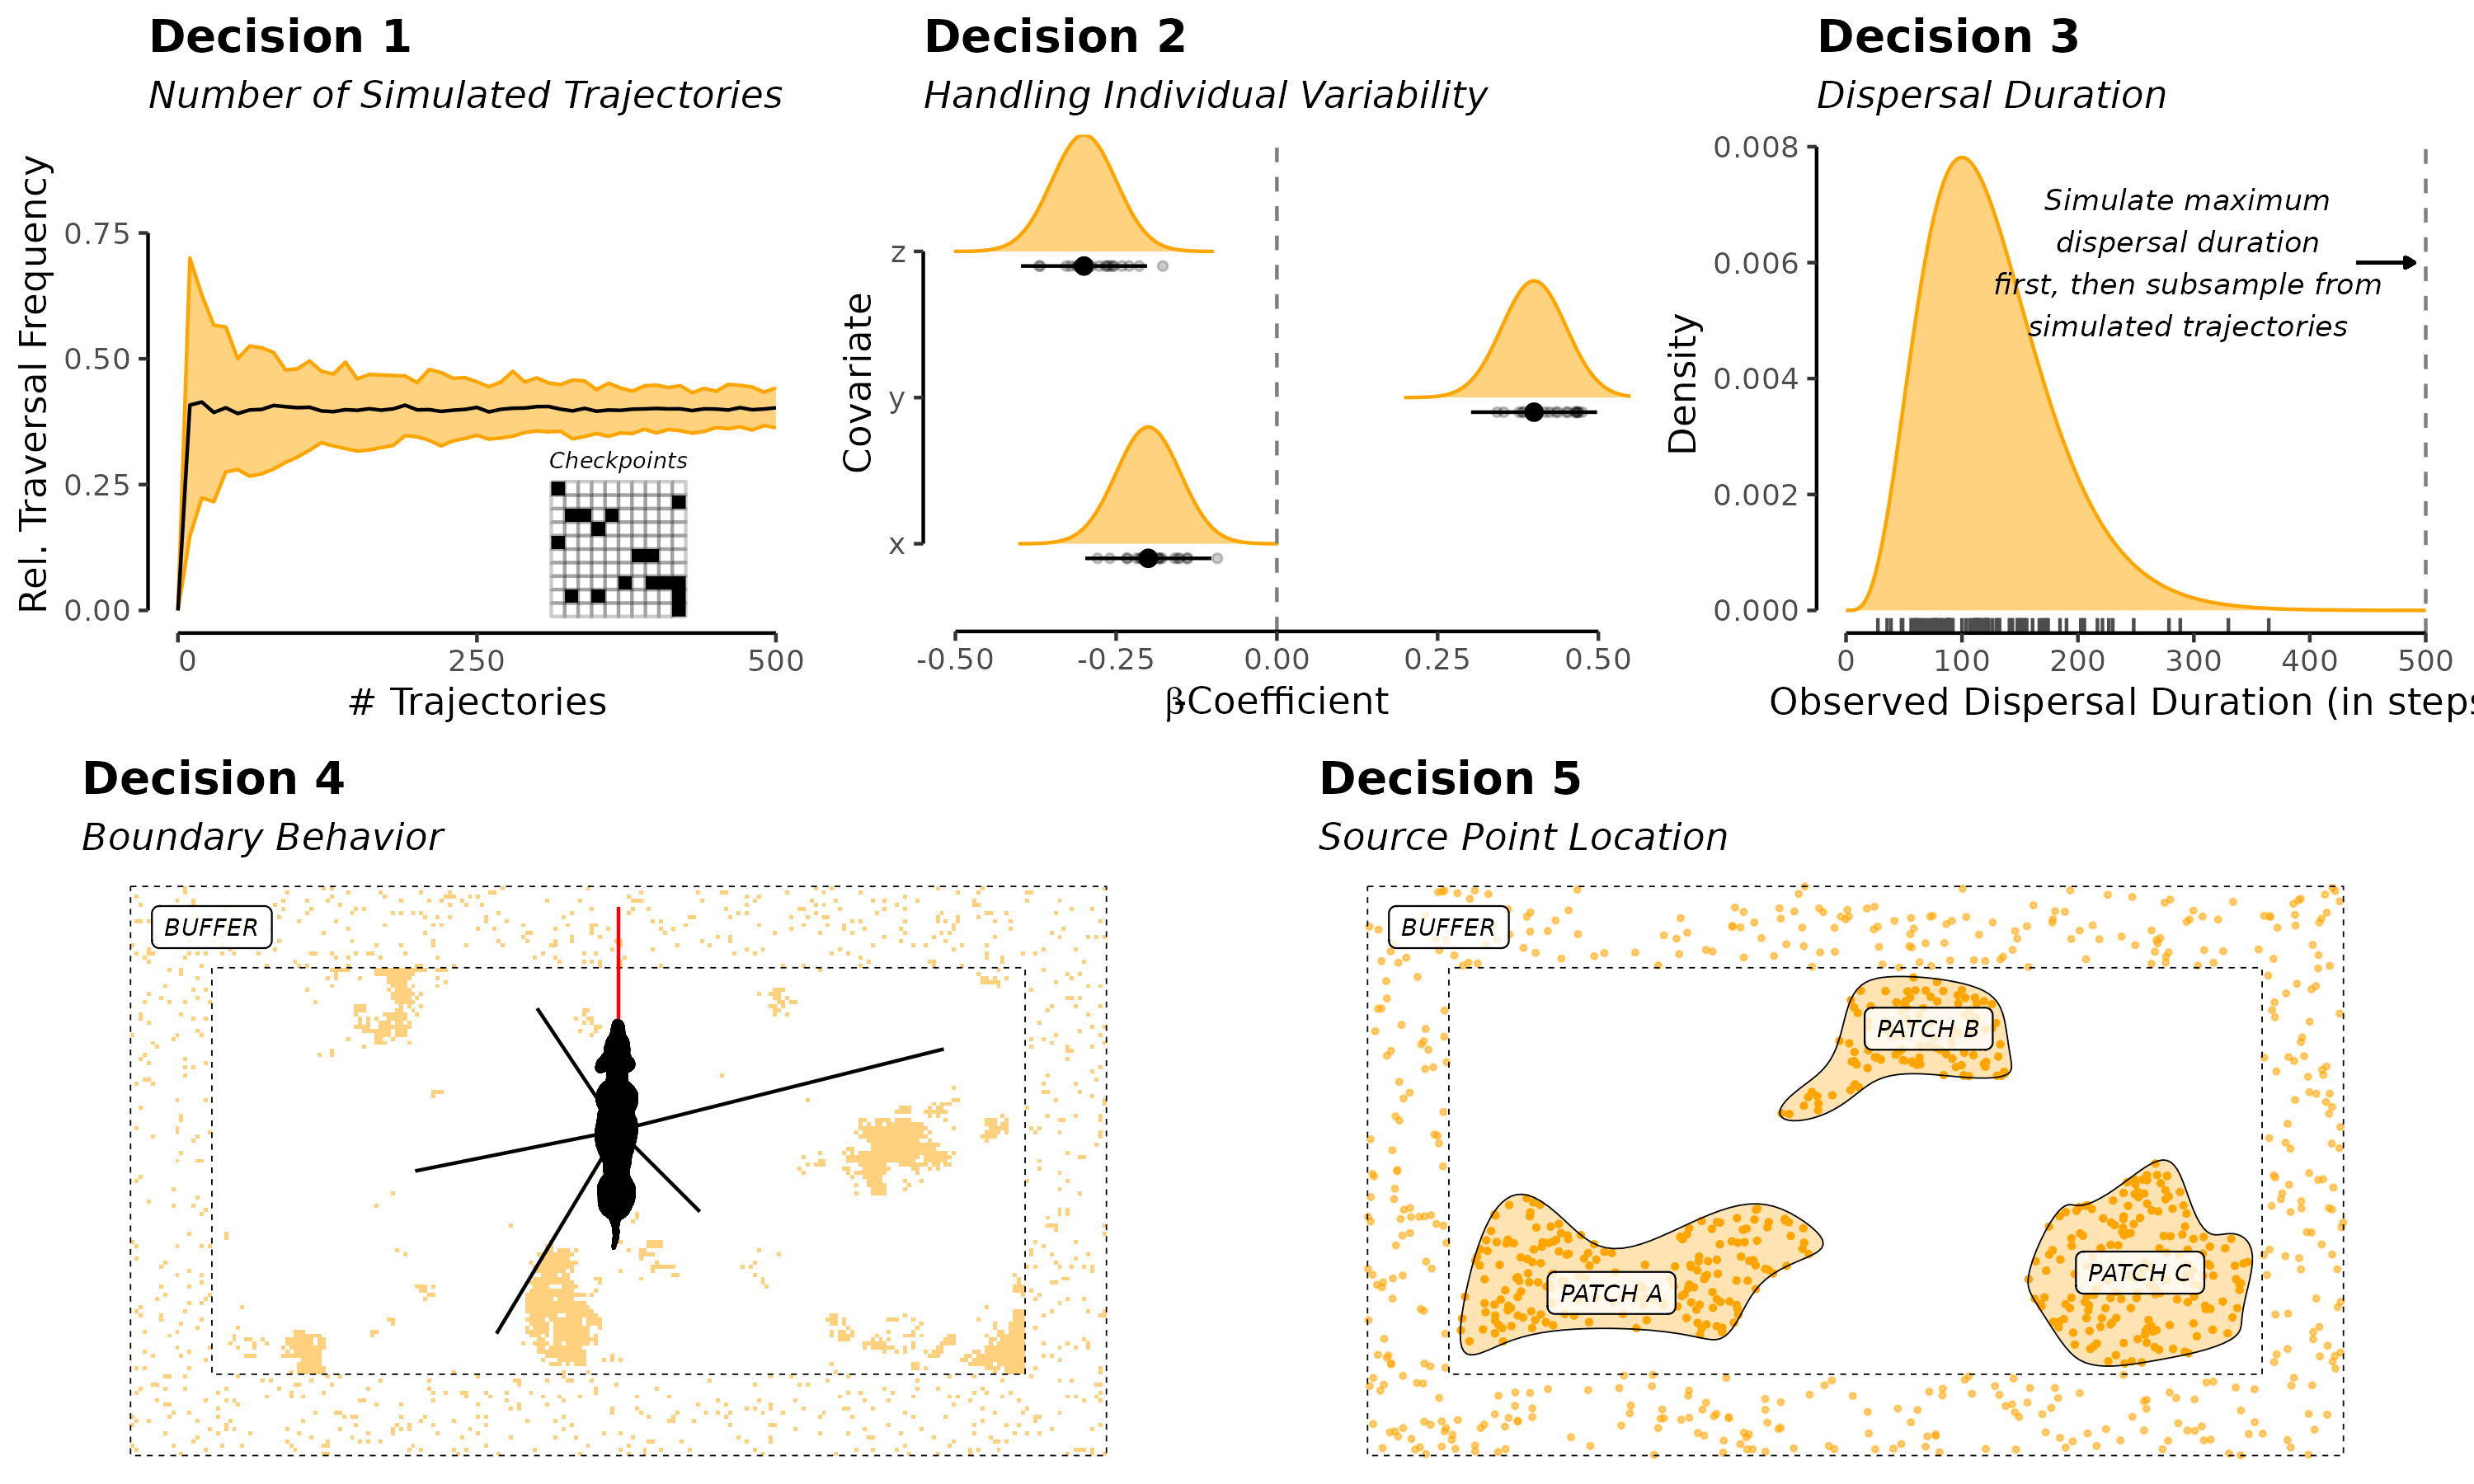
\includegraphics[width=\textwidth]{99_ModelingDecisions.png}
  \caption{Five major modeling decisions that a researcher needs to consider
  when simulating dispersers to assess landscape connectivity. (1) Number of
  simulated trajectories. (2) Handling individual variation: we used point
  estimates when simulating dispersers, assuming that there was no individual
  variation. Alternatively, however, one could draw preferences for each
  simulated individually based on model uncertainty. (3) Dispersal duration.
  While one could draw the number of simulated steps based on observed dispersal
  events, we opted for an alternative and simulated each individual for 2'000
  steps, which was at the upper end of observed dispersal durations. This allows
  to easily shorten the generated trajectories afterwards and to investigate the
  sensitivity of results with regards to the dispersal duration. (4) Boundary
  behavior. We allowed dispersers to leave and re-enter the main study area
  through a buffer zone with randomized covariate values. Alternatively, one
  could discard transgressing random steps, thereby forcing dispersers to remain
  within the study area or simply terminate the simulation, assuming the
  individual has disappeared. (5) Source point location. The location of source
  points should optimally be biologically informed. For our simulation, we
  placed source points within protected areas large enough to sustain viable
  wild dog populations. Conceivable alternatives include placing source points
  according to a habitat suitability model or based on abundance information.
  Importantly, one must also consider potential immigrants from outside the main
  study area.}
  \label{ModelingDecisions}
\end{figure}

Despite the benefits that simulations from ISSFs offer, we also want to confer
some of the non-trivial modeling decisions involved. In particular, we will
discuss five modeling decisions (\Cref{ModelingDecisions}): (1) number of
simulated individuals, (2) location of source points, (3) dispersal duration,
(4) boundary behavior, and (5) how to handle individual variability.

(1) When simulating dispersal using ISSFs, the modeler needs to decide on the
number of simulated individuals. This decision includes the \textit{absolute}
number of simulated individuals across the entire study area, as well as the
\textit{relative} number of simulated individuals per spatial entity (e.g.
protected area, habitat patch, source point). With respect to the
\textit{absolute} number of simulated individuals, a higher number is always
desirable, as each additional disperser provides novel information about
landscape connectivity. Of course this comes at the cost of computational
efficiency, such that a trade-off needs to be managed. We propose to handle this
trade-off by defining a target metric and only simulating additional until
convergence in the target metric is observed. Here, we employed the
\textit{relative traversal frequency} across checkpoints as target metric and
found that convergence across all checkpoints was achieved already after 10'500
simulated individuals. With regards to the \textit{relative} number of simulated
individuals, we see several feasible approaches. If corresponding data is
available, one could distribute dispersers in relation to known abundances,
reflecting that population densities are not necessarily homogeneous across
space. Alternatively, one could also distribute dispersers homogeneously, yet
after the simulation weigh each simulated trajectory according to population
densities at the respective source patch. Again this requires information on the
spatial abundance of the focal speciesl. Finally, if such information is
missing, one can distribute dispersers homogeneously across space. This is the
approach that we employed and resulted in larger source areas generating a
larger number of dispersers.

(2) While we simulated dispersal using point estimates from our most
parsimonious movement model but did not investigate the sensitivity of our
results with respect to those estimates. Uncertainty is rather common in
dispersal studies on endangered species, as data tends to be scarce, resulting
in model estimates large confidence intervals \citep{Wiegand.2003,
KramerSchadt.2007}. To address this, one may explore a broader range of
preferences instead of using point estimates initiate dispersers with randomized
preferences with variability imposed by the uncertainty in the movement model.
We therefore urge future studies to investigate the sensitivity of ISSF
simulations with respect to estimated preferences.

(3) When employing ISSFs to simulate dispersers, one also needs to decide on
meaningful dispersal durations (i.e. number of simulated steps). If
corresponding data is available, dispersal durations could be sampled from
observed events, such that each individual would only be simulated until its
assigned dispersal duration has been achieved. Due to the low number of observed
dispersal events and due to the great variability in wild dogs' dispersal
distances \citep{DaviesMostert.2012, Masenga.2016, Cozzi.2020} we opted against
this approach. Instead, we simulated individuals for 2'000 steps, which is at
the upper end of observed dispersal durations and may have resulted in an overly
optimistic representation of landscape connectivity. Nevertheless, it is
relatively straight forward to shorten simulated trajectories in order to
investigate the sensitivity of results with regards to the dispersal duration.
Alternatively, if detailed information on settlement behavior is available, the
dispersal simulation could include a settlement submodel, where after each
simulated step the simulated individual decides whether or not to settle, based
the number of realized steps, environmental conditions in the landscape,
abundance of conspecifics or comptetitors etc.

(4) Unless simulated individuals are drawn towards a point of attraction, some
individuals will inevitably approach a map boundary such that some of the
proposed random steps will leave the study area such that no selection score can
be computed. One option to handle this situation would be to simply terminate
the simulation as soon as one of the random steps leaves the study area,
assuming that the simulated animal left the study area and will not return. This
can be problematic when many individuals are initiated close to map boundaries,
especially since a single random step leaving the study area forces termination
of the simulation. As an alternative, one could resample transgressing random
steps until all proposed random steps lie fully within the study area. This will
force simulated dispersers to bounce off those boundaries and remain within the
main study area. Finally, one could also extend the study area by an artificial
buffer zone with randomized covariate values through which dispersers are
allowed to leave and re-enter the main study area. Although dispersers might
still approach the boundary of the buffer, it has been shown that adding an
artifical buffer helps to mitigate edge effects \cite{Koen.2010}. A last
solution that only applies in theoretical applications is to simulate movement
on a torus \citep{Hodel.2021b}.

(5) To initiate the simulation of a disperser, the modeler needs to define a
source point. In some cases, exact locations of source populations are known and
source points can be placed accordingly \citep{Kanagaraj.2013}. Moreover, if
abundance estimates are available, these can be used to inform the relative
number of dispersers initiated at each location. The selection of source points
is thus directly related to the relative number of simulated individuals. Here,
we randomly placed source points within protected areas large enough to sustain
viable wild dog populations. Given that the species primarily survives in these
formally protected areas \citep{Woodroffe.1999, DaviesMostert.2012,
Woodroffe.2012, VanDerMeer.2014} we consider this decision to be appropriate. In
other cases, comparable knowledge may be lacking and it could be more beneficial
to delineate likely source patches based on habitat suitability models (e.g.
\citealp{Squires.2013}). After all, the challenge of selecting meaningful source
points is not unique individual-based simulations also applies to LCPA and
CT. However, as highlighted by \cite{Signer.2017}, the influence of the exact
location of source points decreases as the number of simulated steps is
increased.

\subsection{Conclusion (80\%)}
To this end, we have used data on dispersing wild dogs to exemplify how ISSFs
can be used to parametrize an individual-based movement model that is further
employed to simulate dispersal and examine landscape connectivity. We also
presented three complementary connectivity maps derived from simulated
trajectories, each focused on a different aspect of connectivity. Furthermore,
we discussed the potential advantages and disadvantages of the proposed
framework compared to traditional connectivity modeling techniques such as LCPA
and CT. With this article, we hope to have sparked interest in the uprising
framework of step selection functions for investigating dispersal behavior and
landscape connectivity. Nevertheless, we do not attempt to dismiss the
application of traditional connectivity models by any means. Rather, we propose
to use simulations from ISSF-models as a simple but powerful tool to provide a
more comprehensive understanding of dispersal and landscape connectivity.


%------------------------------------------------------------------------------
%  Further Results to Report
%------------------------------------------------------------------------------
% % Some step length, turning angle comparisons
% On average, step lengths realized by the simulated dispersers (\(\mu_{sl} =
% 2'093\) m, \(\sigma_{sl} = 3'067\)) were slightly shorter than those by observed
% dispersers (\(\mu_{sl} = 2'326\) m, \(\sigma_{sl} = 3'323\)) and simulated
% dispersers moved marginally less directional (\(\mu_{cos(ta)} = 0.057\),
% \(\sigma_{cos(ta)} = 0.071\)) compared to observed dispersers (\(\mu_{cos(ta)} =
% 0.078\), \(\sigma_{cos(ta)} = 0.072\)). These differences in step lengths and
% turning angles can be attributed to minor disparities between habitat conditions
% at the area within which we collected training data and habitat conditions
% within the entire study area.

%------------------------------------------------------------------------------
%  Further Topics to Discuss
%------------------------------------------------------------------------------

% % Simulations for an early warning system?
% Finally, simulations from ISSFs could be utilized as forecasting tool to predict
% the likely whereabouts of GPS collared animals into the near future. In some
% European countries, the reintroduction of large predators, such as bears, lynx,
% and wolves, has triggered emotional discussions and raised public concern
% \citep{Behr.2017}, particularly in areas where locals depend on income from
% free-roaming livestock. An early warning system based on simulations could thus
% serve to inform about potential encounters with large carnivores, such that
% farmers can secure their livestock accordingly. This would hopefully increase
% public acceptance of large predators.

% % Downsides of connectivity?
% Even though connectivity is in general thought to promote population viability,
% it is also related to various aspects that may cause ecological damage, such as
% increased connectivity into human-dominated areas or facilitated spread of
% deadly diseases \citep{Brearly.2013}. Nevertheless, information on the
% relationship between connectivity and the prevalence of deadly diseases in
% African wild dogs is currently lacking.

% % Social landscape
% We have previously attributed the weak significance of distance to water to the
% fact that we did not control for the presence or absence of conspecifics. We
% stick to this reasoning as our expanded model still shows a rather large
% uncertainty around the respective beta coefficients. To better gauge the
% importance and influence of this covariate, future studies will need to control
% for inter- and intra-specific interactions that may explain why and when
% dispersers are attracted to or afraid of waterbodies. \cite{Fortin.2005}, for
% instance, found that elk movement was significantly impacted by the density of
% wolf in the area, such that habitat preferences strictly differed depending on
% the presence or absence of wolves. The decision to settle is likely related to
% the presence or absence of conspecifics. Hence, the exact dispersal duration and
% distance will not be independent of current wild dog densities. In dispersing
% wolves, for instance, the longest dispersal distances have been observed in
% low-density populations \citep{Boyd.2005, Wabakken.2007}. The dispersal duration
% may thus be determined by the by the amount of isolation between subpopulations
% and population densities \citep{DaviesMostert.2012}

% % Can generate multiple metrics
% Another benefit of simulations from ISSFs is that their output can be processed
% using a diverse suite of approaches, each enabling to focus on a different
% aspect of connectivity. the results from LCPA and CT, on the other hand, are
% usually restricted to single ``conductance'' maps. By turning simulated
% trajectories into a network, for instance, researchers can capitalize on
% concepts from network theory and calculate network metrics that are pertinent to
% landscape connectivity \citep{BastilleRousseau.2018}. Here, we exemplified
% this by calculating the betweenness metric, highlighting major movement
% corridors. Alternatively, can learn about inter-patch connectivity and potential
% source-sink dynamics between patches \citep{Ferreras.2001, Revilla.2004,
% Kanagaraj.2013} based on simulated dispersal trajectories. Ultimately, by
% accounting for habitat- and movement preferences of the focal species,
% simulations from ISSFs are capable of rendering the behavioral ecology of the
% focal species in detail, thereby permitting a more functional view on
% connectivity that is not solely driven by the landscape structure and distances
% between patches \citep{Gustafson.1996, Gardner.2004, Graf.2007,
% KramerSchadt.2004, Revilla.2004, Revilla.2008, Kanagaraj.2013}.

% % We did not validate all of our predictions
% Even though our simulations generated several interesting results, most of them
% need to be validated using independent data. We learned that between some
% national parks asymmetries between the number of ingoing and outgoing dispersers
% exist, suggesting that some patches act as sinks, whereas others serve as
% sources for dispersers.

\section{Authors' Contributions}
D.D.H., D.M.B., A.O. and G.C. conceived the study and designed methodology;
D.M.B., G.C., and J.W.M. collected the data; D.D.H. and D.M.B. analysed the
data; G.C. and A.O. assisted with modeling; D.D.H., D.M.B., and G.C. wrote the
first draft of the manuscript and all authors contributed to the drafts at
several stages and gave final approval for publication.

\section{Data Availability}
GPS movement data of dispersing coalitions will be made available on dryad at
the time of publication. Access to all R-scripts is provided through Github.

\section{Acknowledgements}
We thank the Ministry of Environment and Tourism of Botswana for granting
permission to conduct this research. We thank C. Botes, I. Clavadetscher, and G.
Camenisch for assisting with wild dog immobilizations. We also thank B. Abrahms
for sharing her data of three dispersing wild dogs. Furthermore, we are indebted
to Johannes Signer for assisting with the simulation algorithm. This study was
funded by Basler Stiftung für Biologische Forschung, Claraz Foundation, Idea
Wild, Jacot Foundation, National Geographic Society, Parrotia Stiftung, Stiftung
Temperatio, Wilderness Wildlife Trust Foundation, Forschungkredit der
Universität Zürich, and a Swiss National Science Foundation Grant
(31003A\_182286) to A. Ozgul.

\newpage
\begingroup
\singlespacing
\bibliography{Literatur}
\endgroup

\end{document}
